In the final section of this thesis, we will explore the fANOVA decomposition visually. This will provide better understanding for how fANOVA components behave in different scenarios; also if fANOVA should enhance interpretability, it is important to have visualizations of it. We will first revisit our running example and then explore some other functions.
\subsection{Comparison of Decompositions}
Recall our running example:
$$h(x_1, x_2) = x_1 + 2 x_2 + x_1 x_2,$$
with polynomial coefficients: $a_0 = 0$, $a_1 = 1$, $a_2 = 2$, $a_{11} = 0$, $a_{22} = 0$, $a_{12} = 1$.
Under independent inputs ($\rho = 0$), the fANOVA components are given by:
\begin{align*}
y_{\emptyset} &= 0, \\
y_1(x_1) &= x_1\\
y_2(x_2) &= 2x_2\\
y_{12}(x_1, x_2) &= x_1x_2,
\end{align*}
visualized in \autoref{fig:running_ex_independent}. As expected, we observe simple linear functions and a regular symmetric contour plot.
% Input: MVN, centred, independent
\begin{figure}[htpb]
    \centering
    \begin{subfigure}[t]{0.49\textwidth}
        \centering
        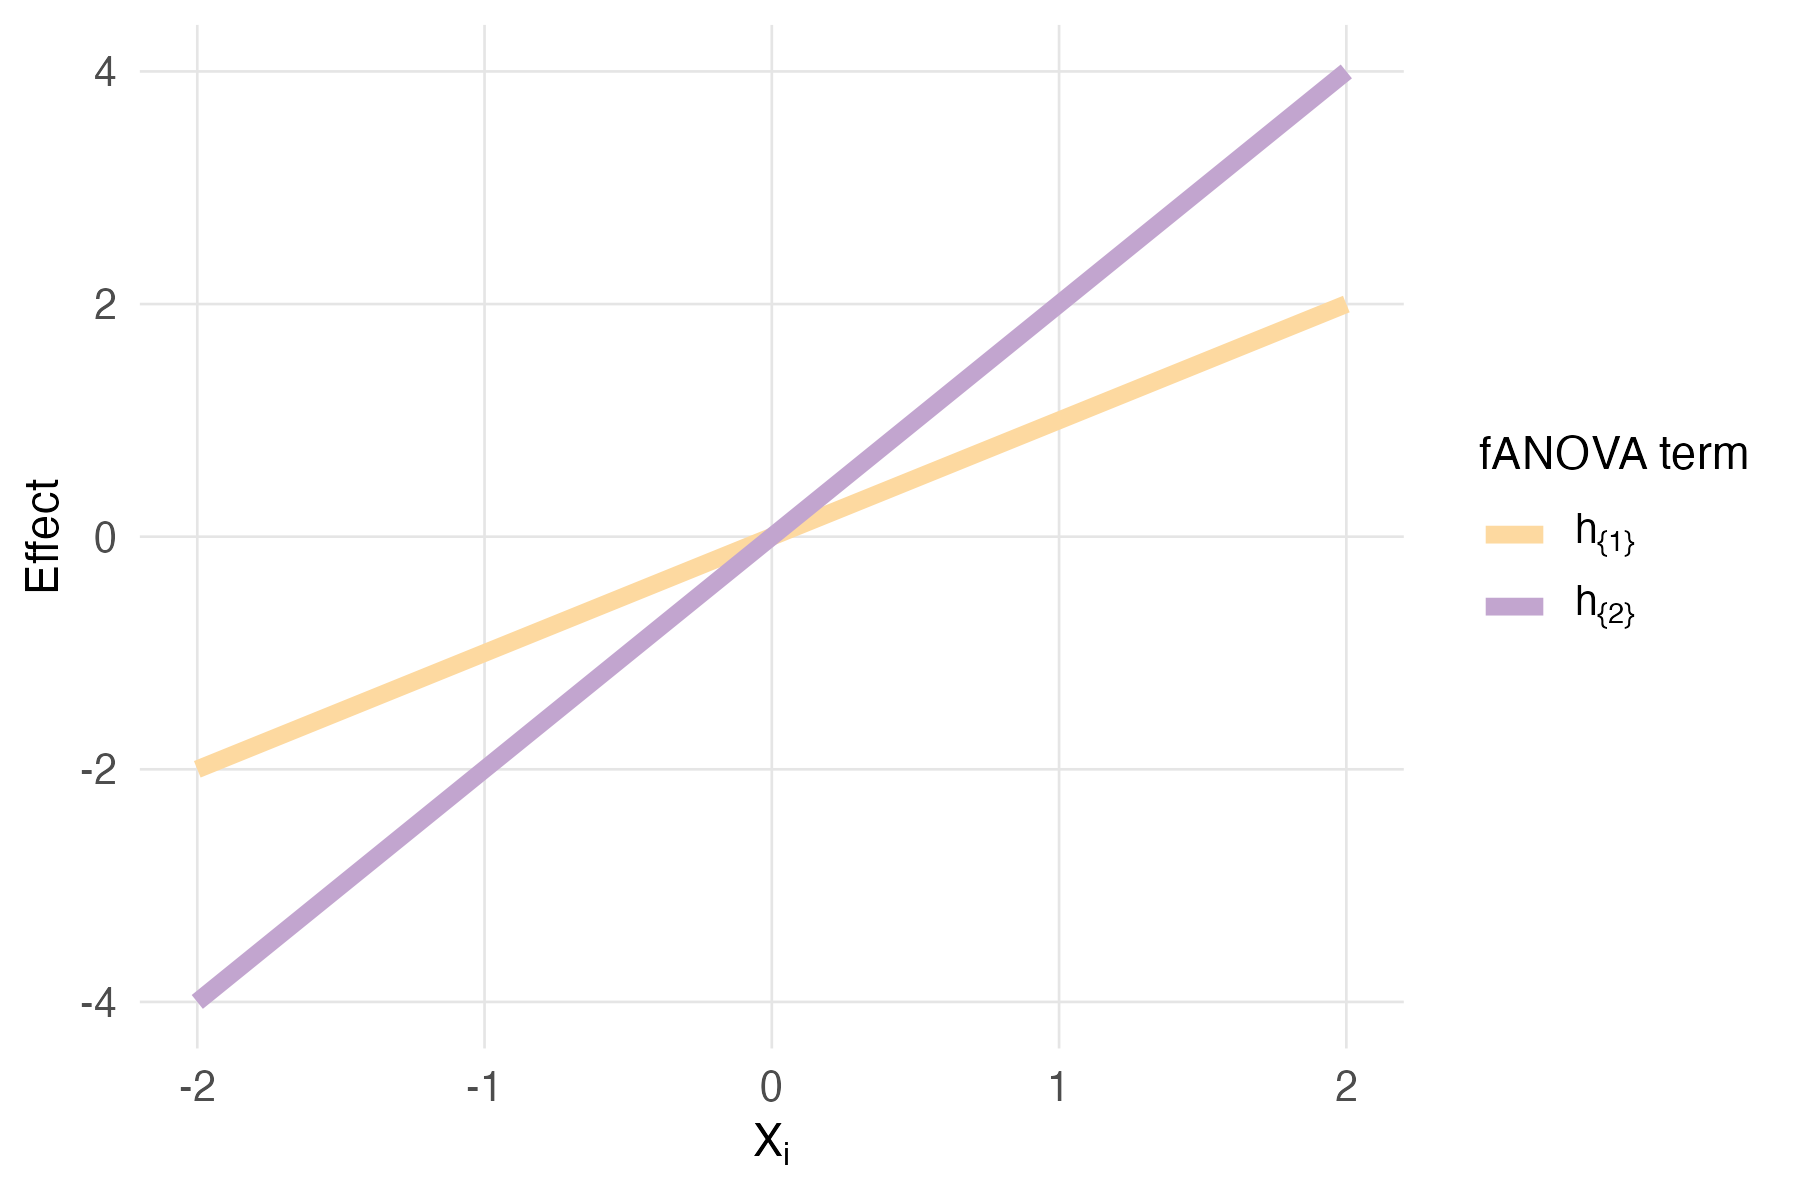
\includegraphics[width=\textwidth]{images/experiment_section/running_example_a1p10_a2p20_a11p00_a22p00_a12p10_rhop00_main.png}
    \end{subfigure}%
    \hfill
    \begin{subfigure}[t]{0.49\textwidth}
        \centering
        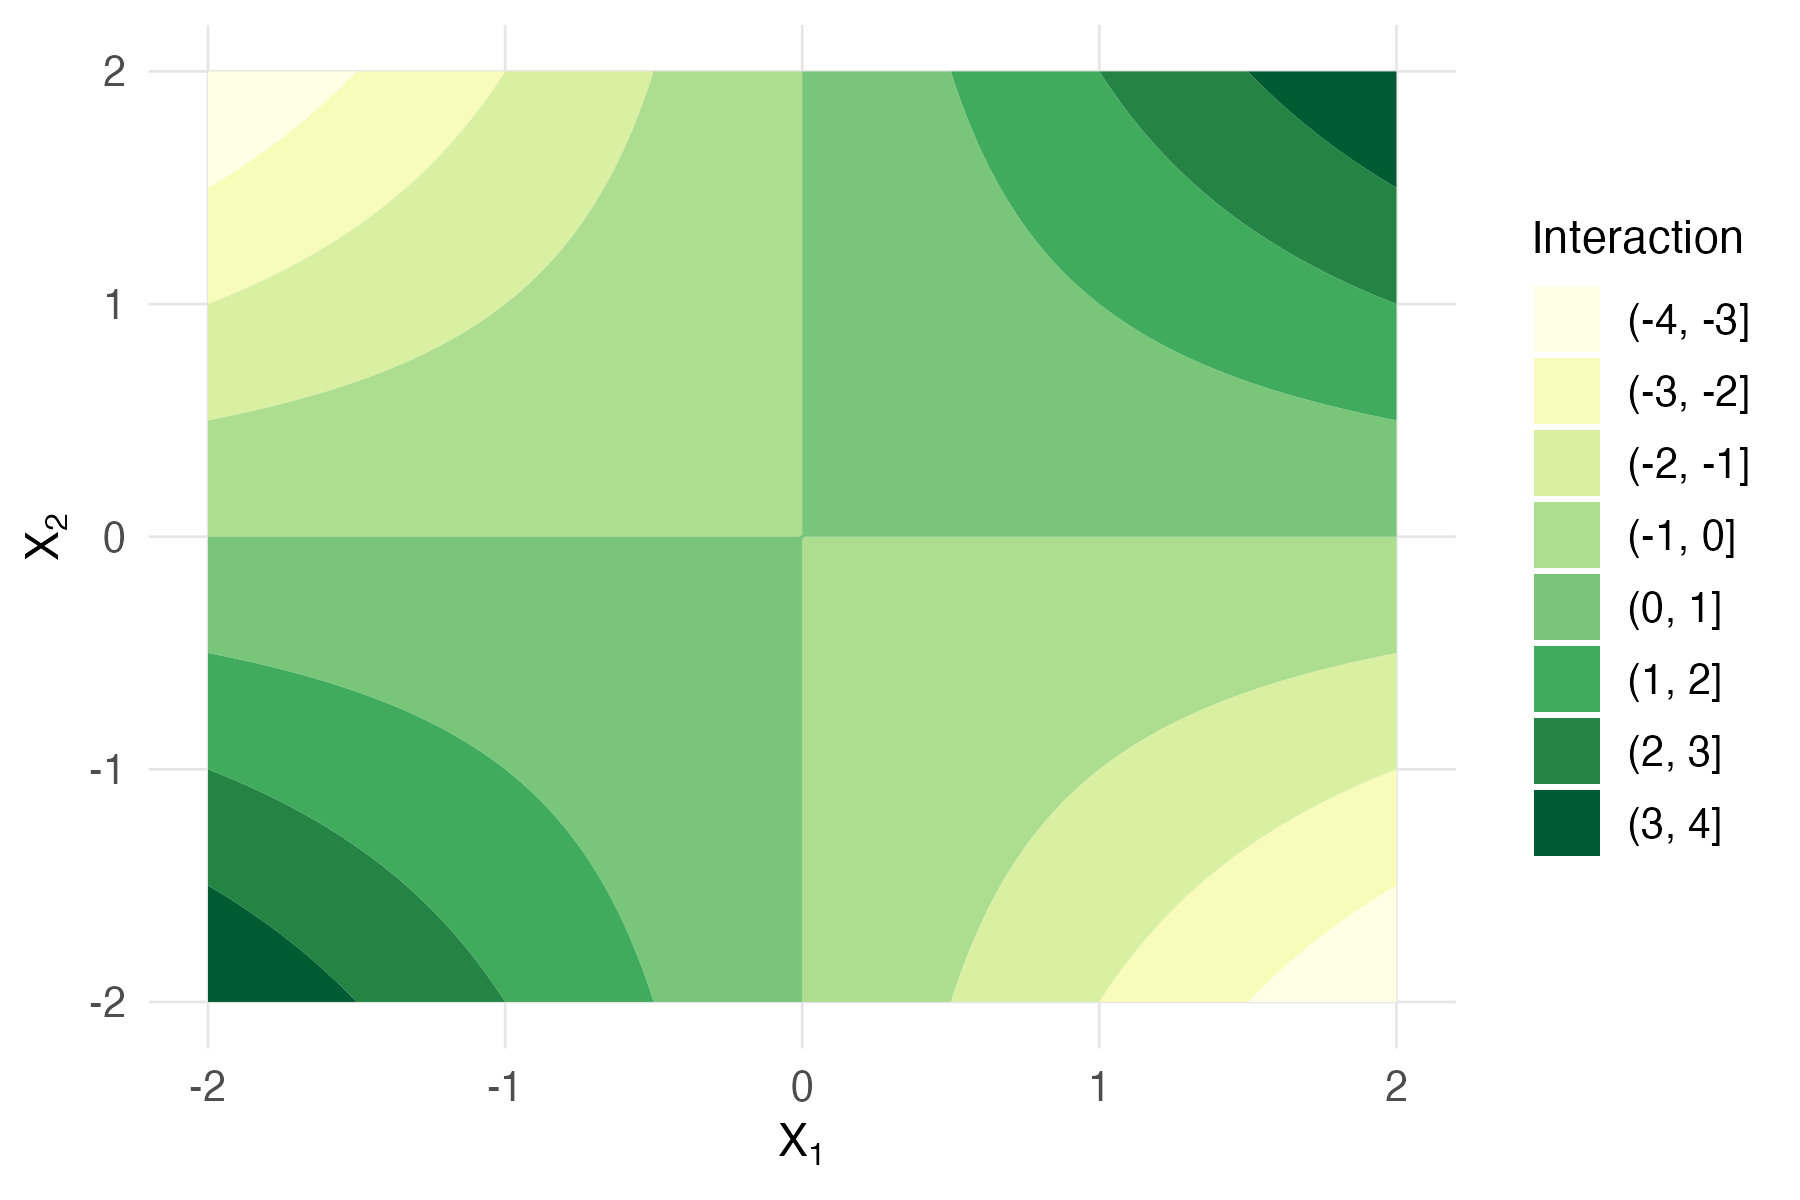
\includegraphics[width=\textwidth]{images/experiment_section/running_example_a1p10_a2p20_a11p00_a22p00_a12p10_rhop00_interaction.png}
    \end{subfigure}
    \caption{Main effects (left) and interaction effect (right) of the fANOVA decomposition for $h(x_1, x_2) = x_1 + 2 x_2 + x_1 x_2$ with independent inputs.}
    \label{fig:running_ex_independent}
\end{figure}

Now we assume $\rho = 0.5$. In attempt to compute the fANOVA terms under dependent inputs, we calculated the following effects, which are in reality the components of the Hoeffding decomposition:

\begin{align*}
\tilde{y}_0 &= a + 0.5 \\[3pt]
\tilde{y}_1(x_1) &= 2x_1 + 0.5x_1^2 - 0.5 \\[3pt]
\tilde{y}_2(x_2) &= 2.5x_2 + 0.5x_2^2 - 0.5 \\[3pt]
\tilde{y}_{12}(x_1,x_2) &= x_1x_2 - x_1 - 0.5x_2 - 0.5x_1^2 - 0.5x_2^2 + 0.5,
\end{align*}
which are visualized in \autoref{fig:hoeffding_rho05}. The main effects are parabolic, and the interaction term seems to be non-symmetric.
\begin{figure}[htpb]
    \centering
    \begin{subfigure}[t]{0.49\textwidth}
        \centering
        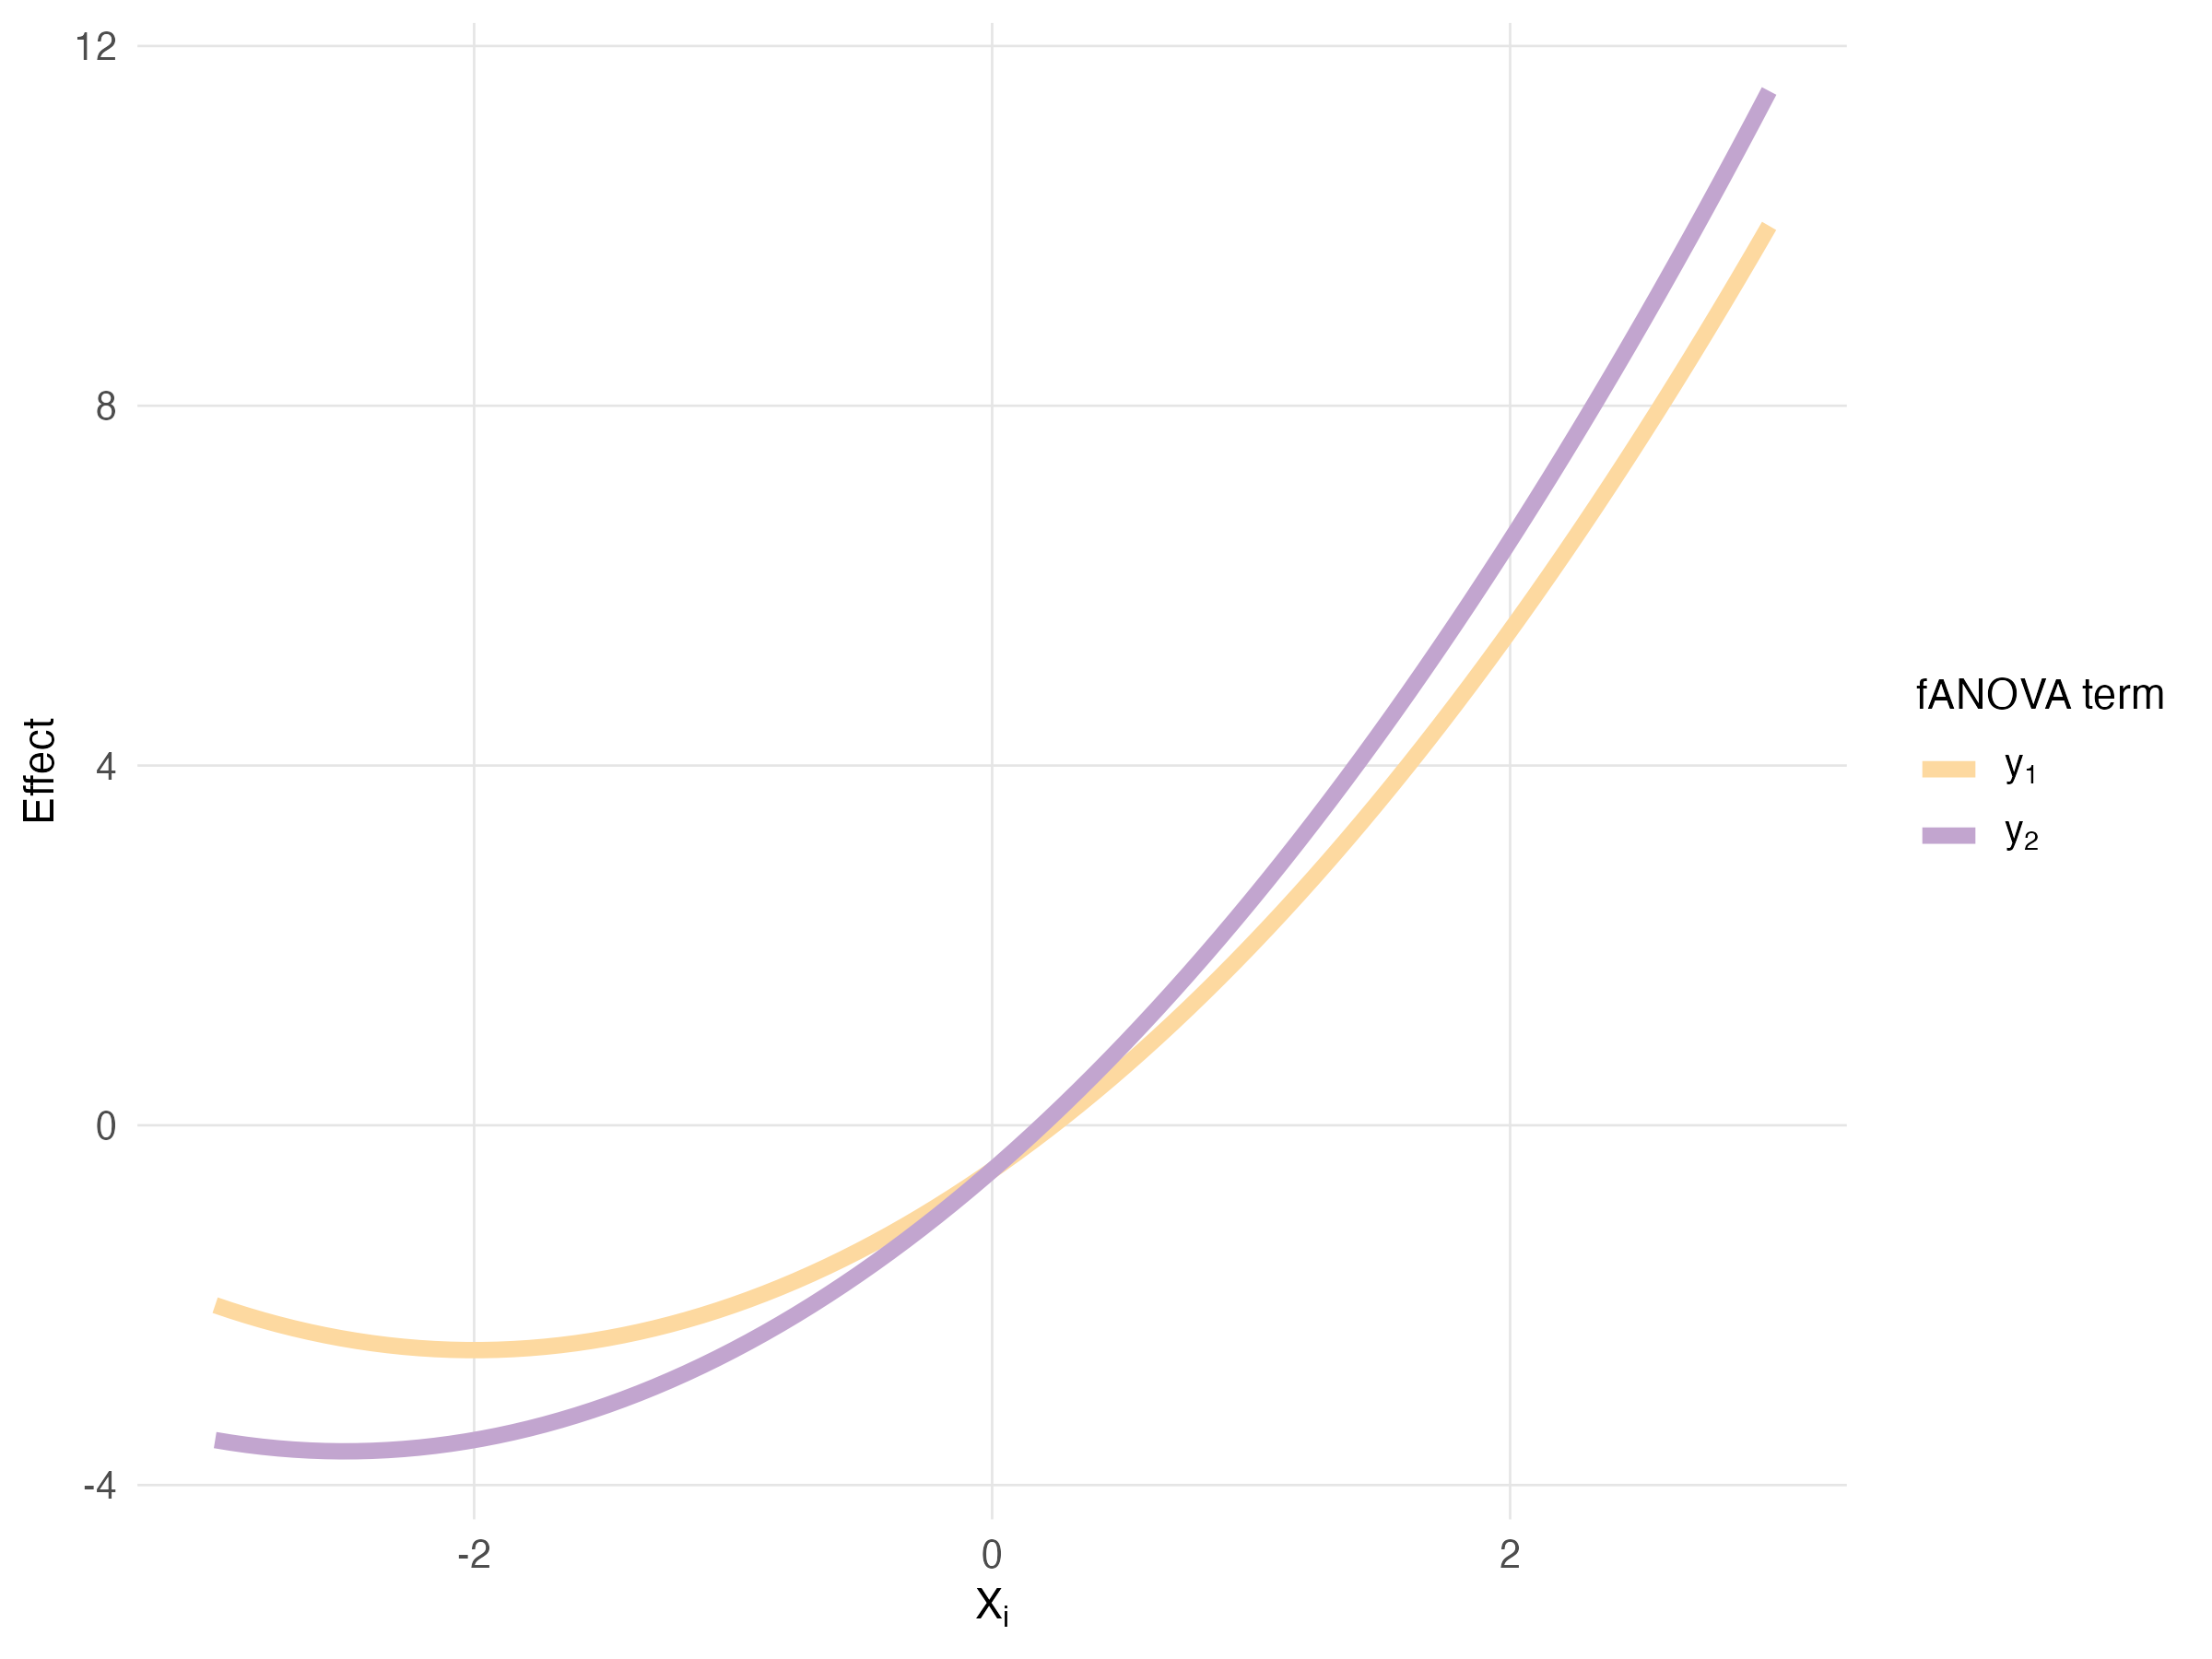
\includegraphics[width=\textwidth]{images/experiment_section/hoeffding_rho05_main.png}
    \end{subfigure}%
    \hfill
    \begin{subfigure}[t]{0.49\textwidth}
        \centering
        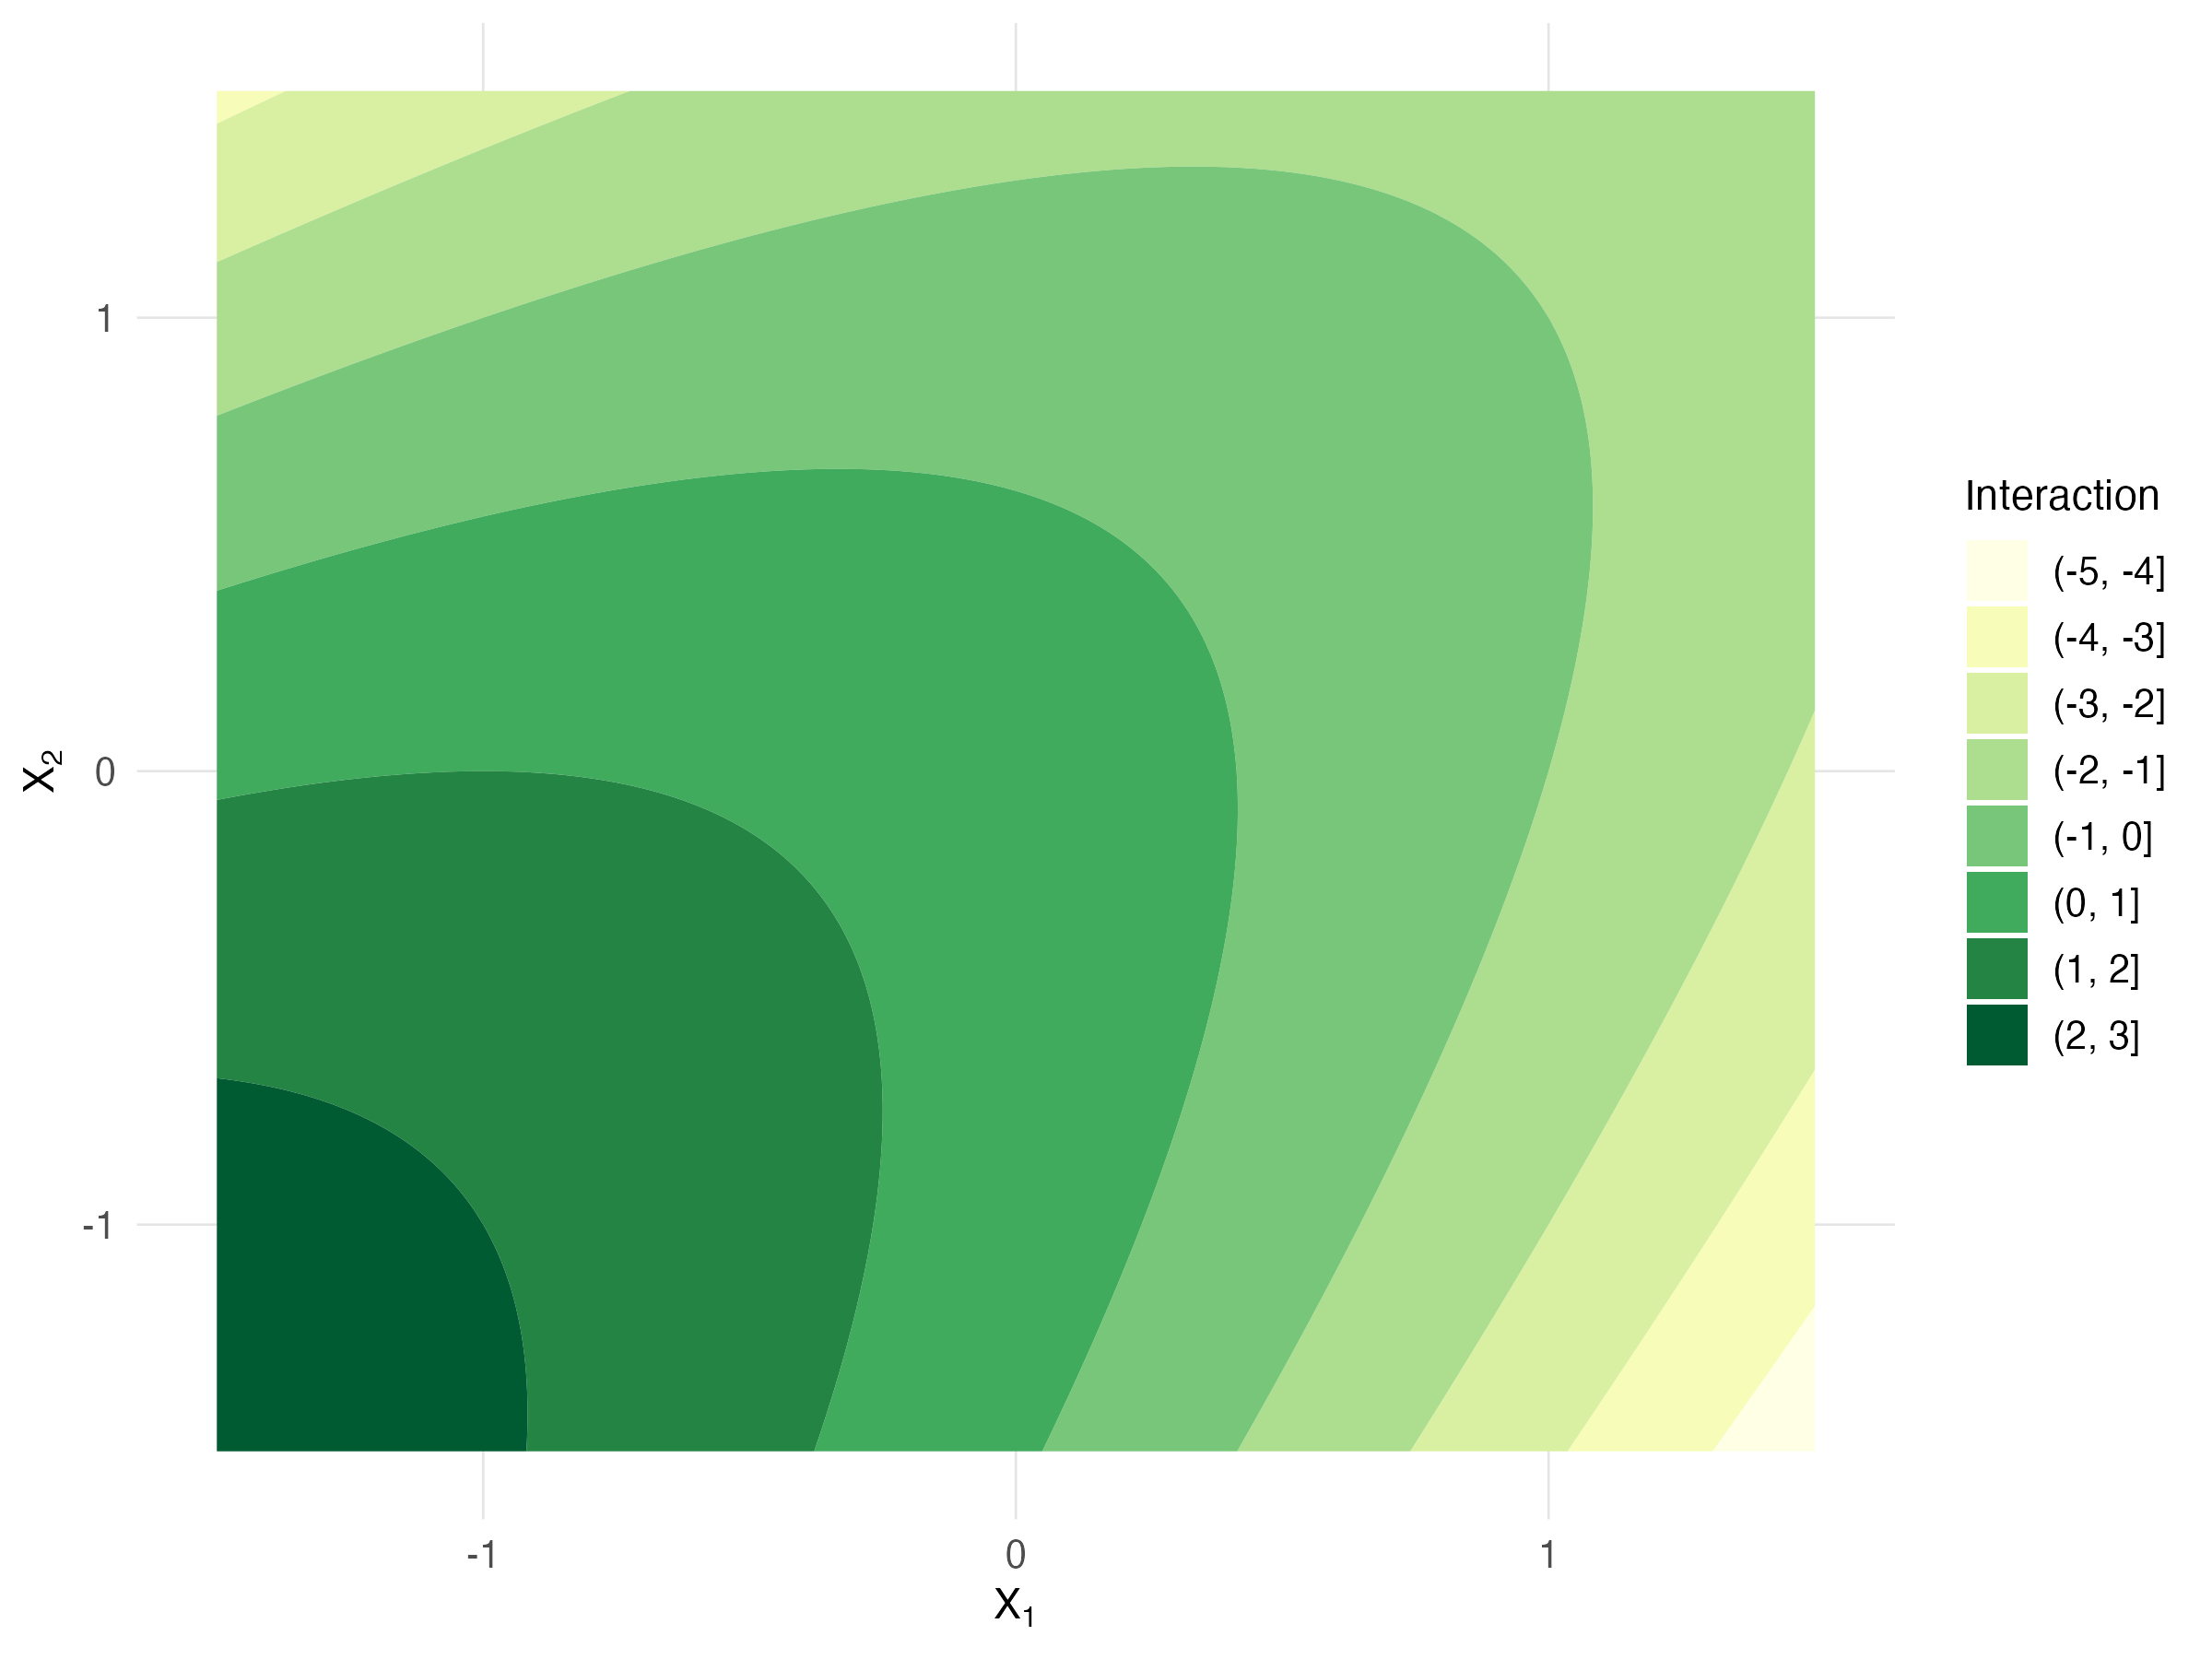
\includegraphics[width=\textwidth]{images/experiment_section/hoeffding_rho05_interaction.png}
    \end{subfigure}
    \caption{Main effects (left) and interaction effect (right) of the Hoeffding decomposition for $g(x_1, x_2) = x_1 + 2 x_2 + x_1 x_2$ with dependent inputs, $\rho = 0.5$.}
    \label{fig:hoeffding_rho05}
\end{figure}
The true fANOVA components under $\rho = 0.5$ are given by:
\begin{align*}
y_0 &= 0.5 \\[3pt]
y_1(x_1) &= x_1 + 0.4\,(x_1^2 - 1)
        = x_1 + 0.4x_1^2 - 0.4 \\[3pt]
y_2(x_2) &= 2x_2 + 0.4\,(x_2^2 - 1)
        = 2x_2 + 0.4x_2^2 - 0.4 \\[3pt]
y_{12}(x_1,x_2) 
&= -\Big( 0.4(x_1^2 + x_2^2) - x_1 x_2 - 0.3 \Big) \\[3pt]
&= -0.4x_1^2 - 0.4x_2^2 + x_1 x_2 + 0.3.
\end{align*}
These are visualized in \autoref{fig:running_ex_dependent}.
% Input: MVN, dependent, rho = 0.5
\begin{figure}[htpb]
    \centering
    \begin{subfigure}[t]{0.49\textwidth}
        \centering
        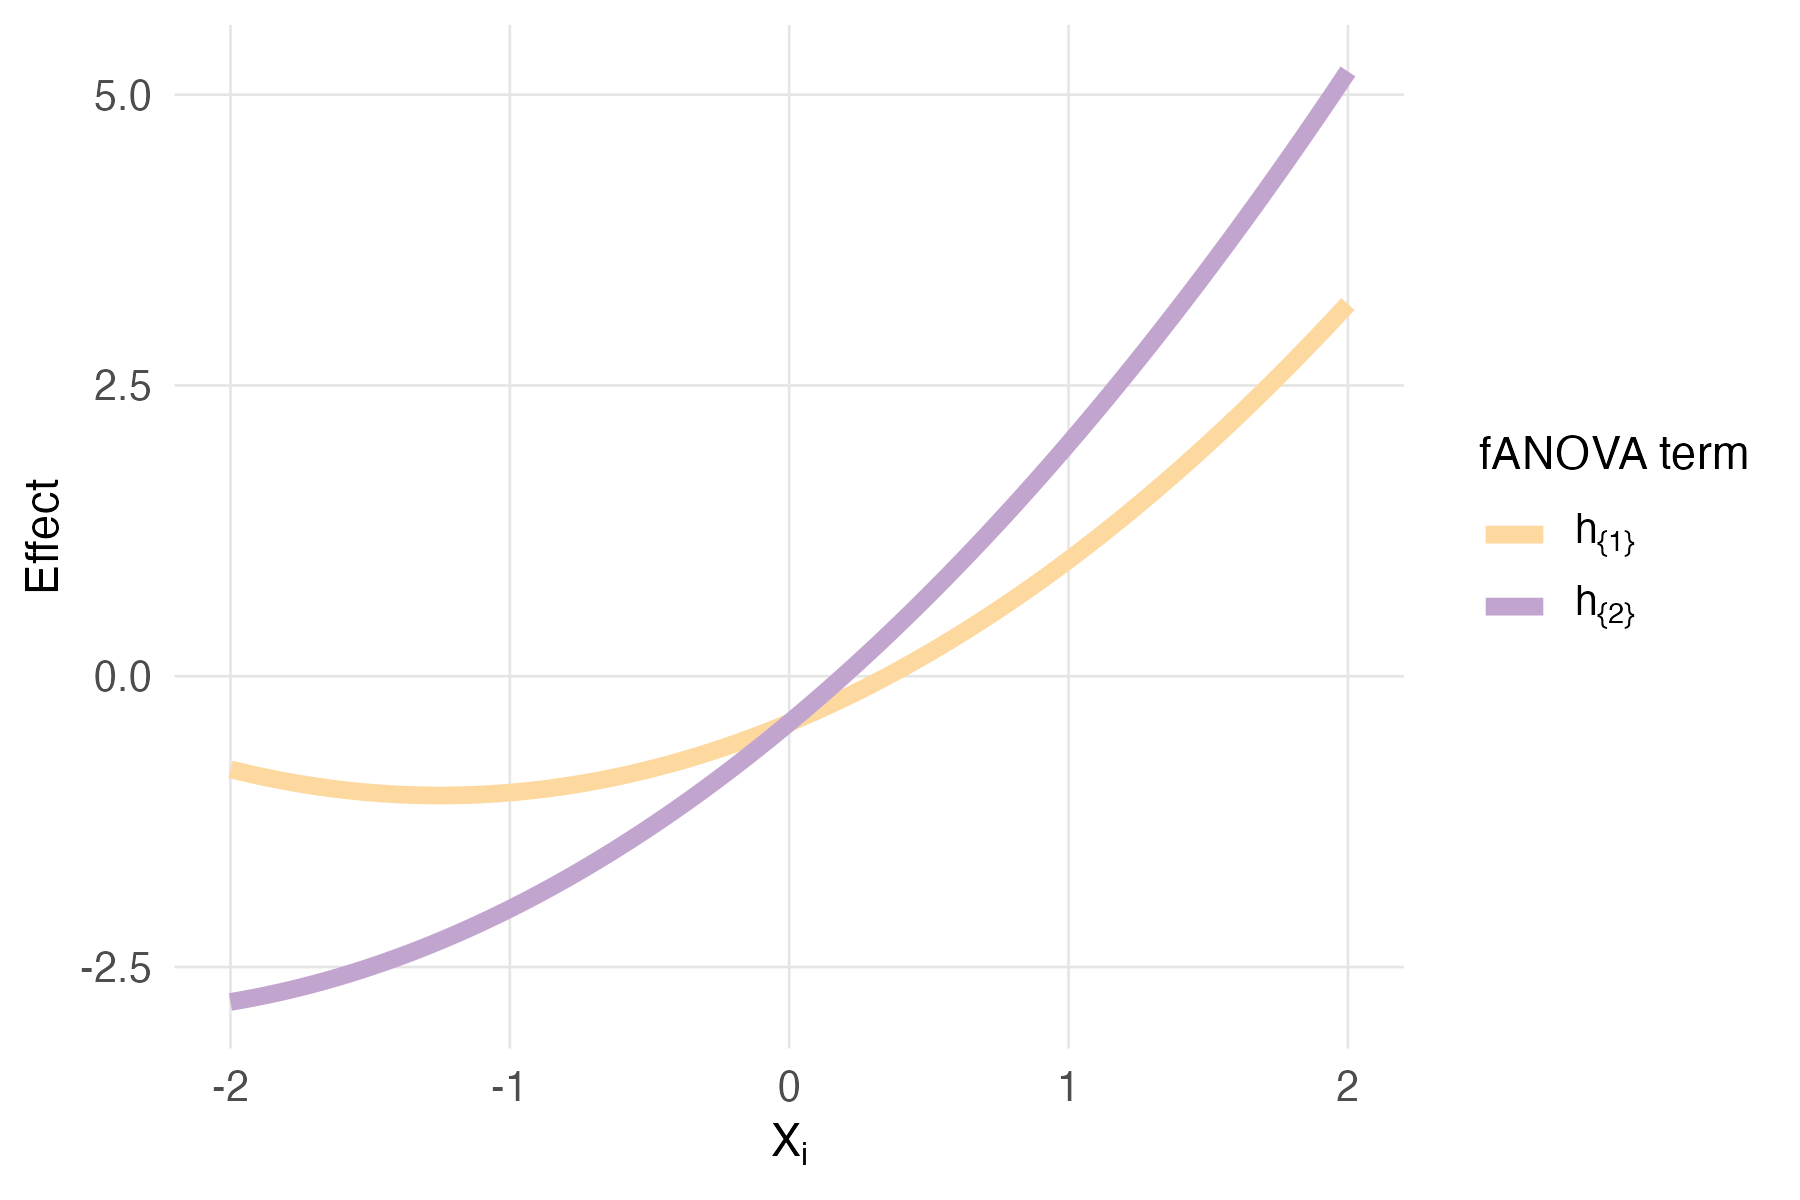
\includegraphics[width=\textwidth]{images/experiment_section/running_example_a1p10_a2p20_a11p00_a22p00_a12p10_rhop05_main.png}
    \end{subfigure}%
    \hfill
    \begin{subfigure}[t]{0.49\textwidth}
        \centering
        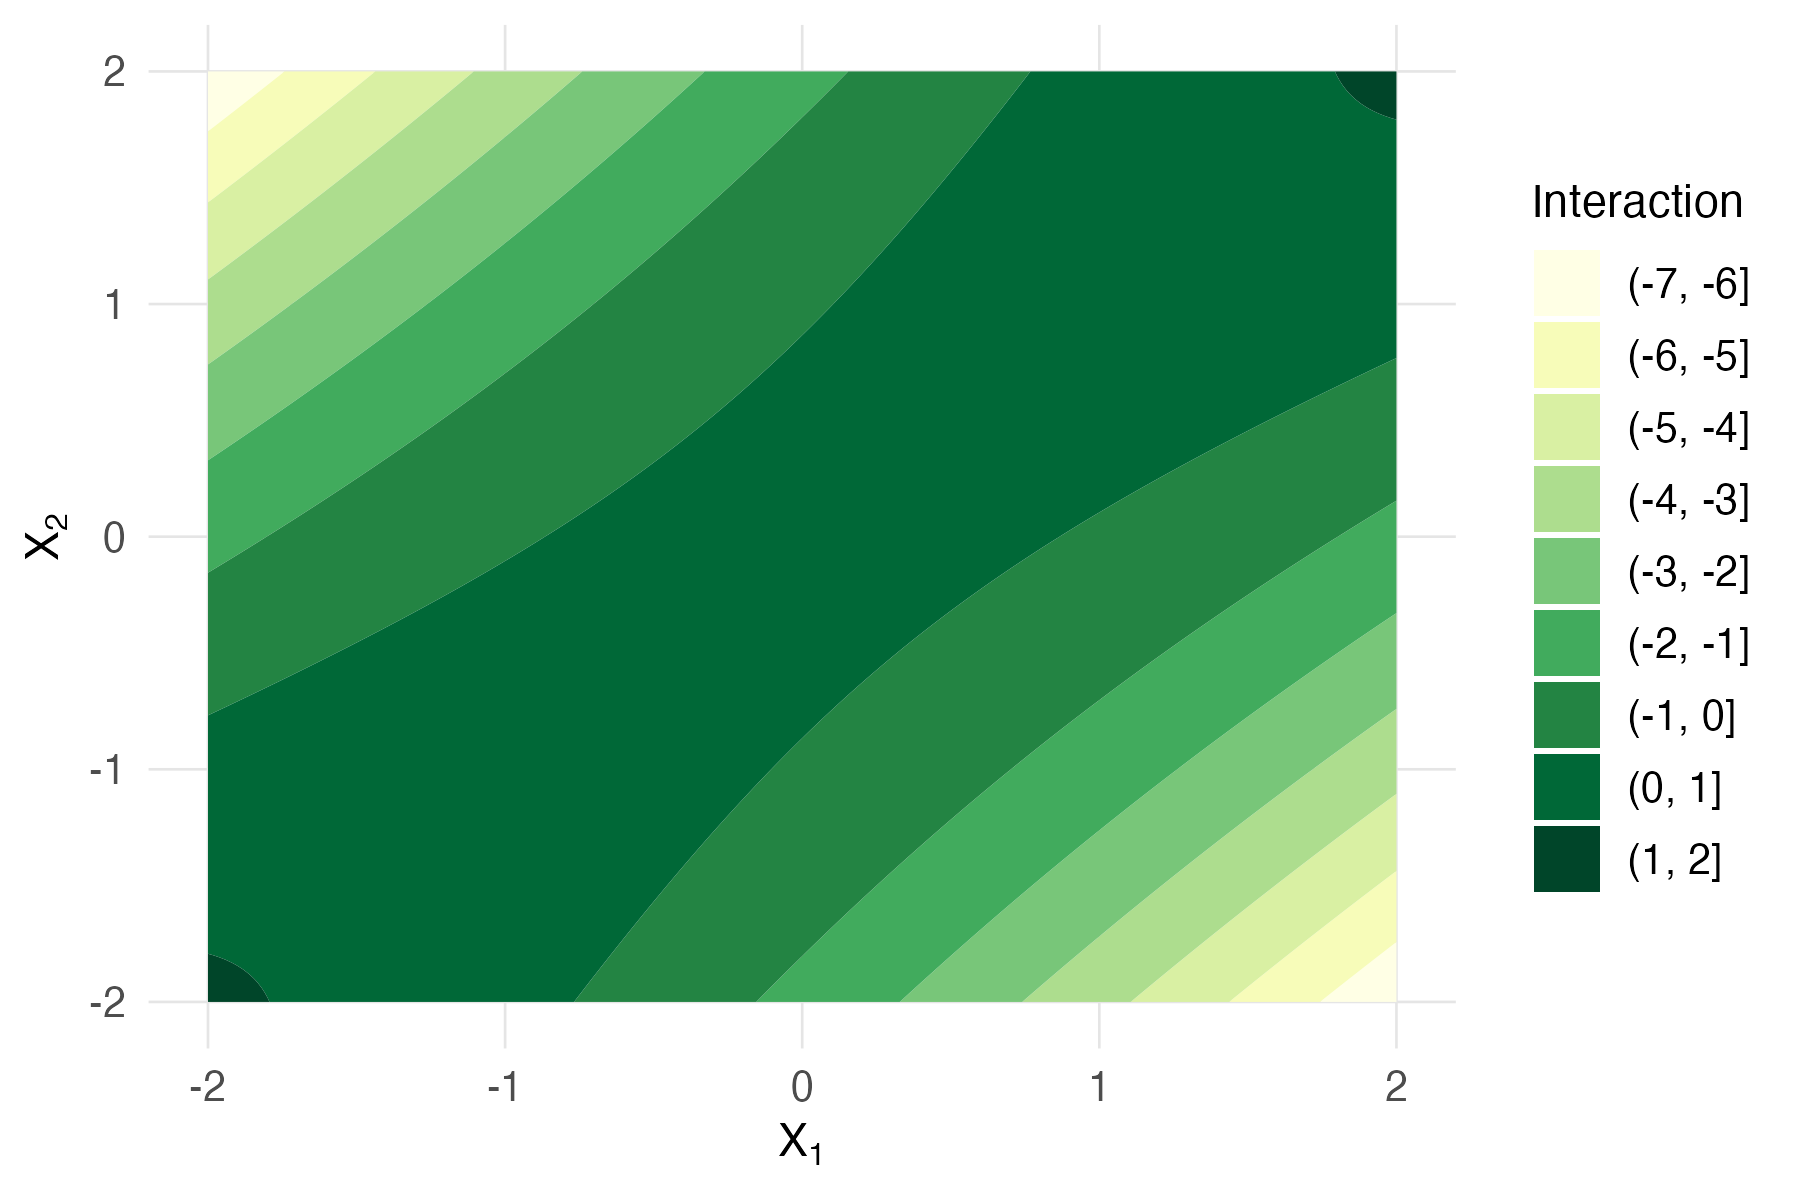
\includegraphics[width=\textwidth]{images/experiment_section/running_example_a1p10_a2p20_a11p00_a22p00_a12p10_rhop05_interaction.png}
    \end{subfigure}
    \caption{Main effects (left) and interaction effect (right) of the generalized fANOVA decomposition for $g(x_1, x_2) = x_1 + 2 x_2 + x_1 x_2$ with dependent inputs, $\rho = 0.5$.}
    \label{fig:running_ex_dependent}
\end{figure}
Interestingly, the parabolic form of the main effects is similar between Hoeffding and fANOVA, but the interaction effects diverge notably.\par
Our running example included linear effects of both input variables and the interaction term. For the remainder of this section, we will explore other representative scenarios, we can build within the scaffold of a bivariate two degree polynomial.

\subsection{Comparison of Functions}
\subsubsection*{Scenario: Linear}
First, we consider two-degree polynomials of the form:
$$g_1(x_1, x_2) = a_1 x_1 + a_2 x_2.$$
We can immediately read of the fANOVA components or use the general set of fANOVA components for a two degree polynomial in \autoref{eq:fanova_components_2D_polynomial} which simplify for $g_1$ to:
\begin{align*}
    y_1(x_1) &= a_1 x_1 \\
    y_2(x_2) &= a_2 x_2.
\end{align*}
This is an even simpler case than our running example. The function can solely be described by linear main effects, while no interaction effects is present (\autoref{fig:linear_main_effects}).

\begin{figure}[htpb]
    \centering
    \begin{subfigure}[t]{0.49\textwidth}
        \centering
        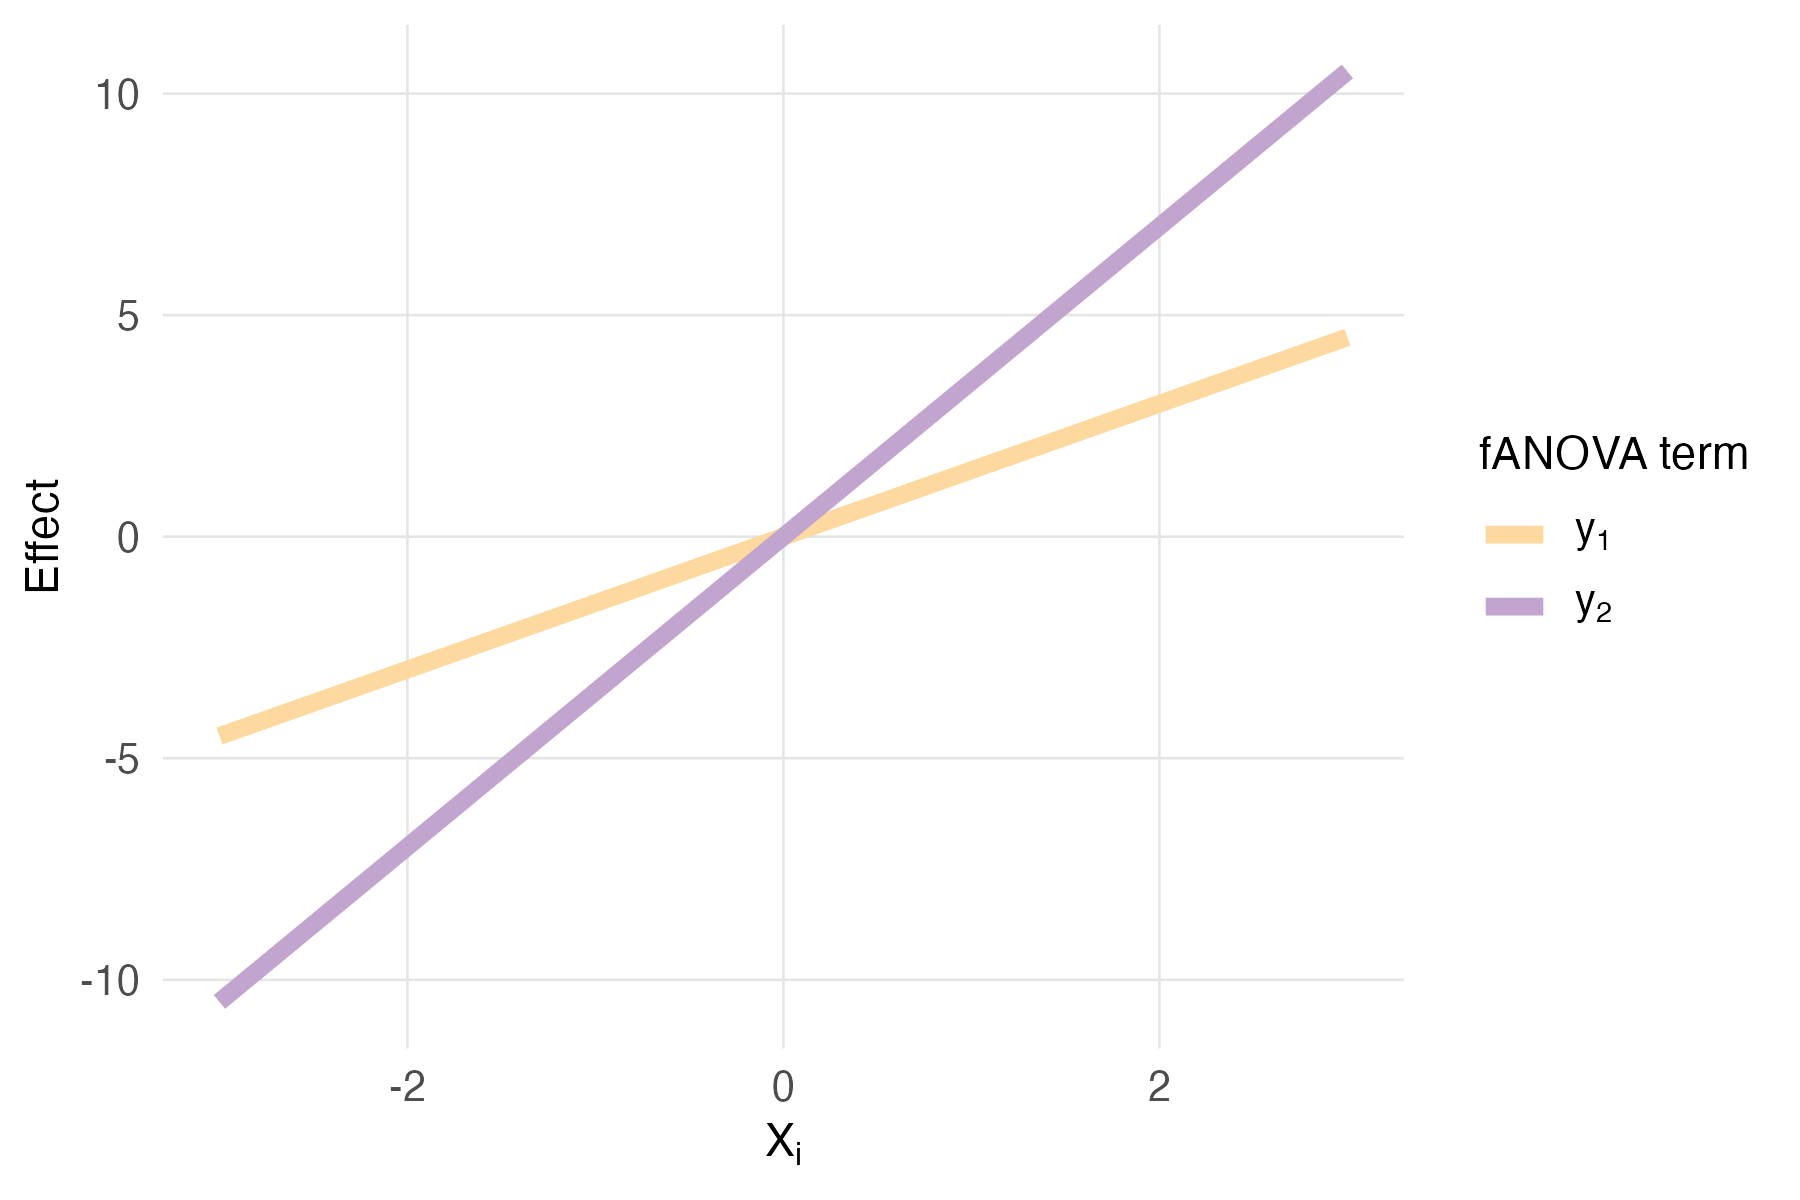
\includegraphics[width=\textwidth]{images/experiment_section/linear_a1p15_a2p35_a11p00_a22p00_a12p00_rhop00_main.png}
        \caption{$a_1 = 1.5$, $a_2 = 3.5$}
    \end{subfigure}%
    \hfill
    \begin{subfigure}[t]{0.49\textwidth}
        \centering
        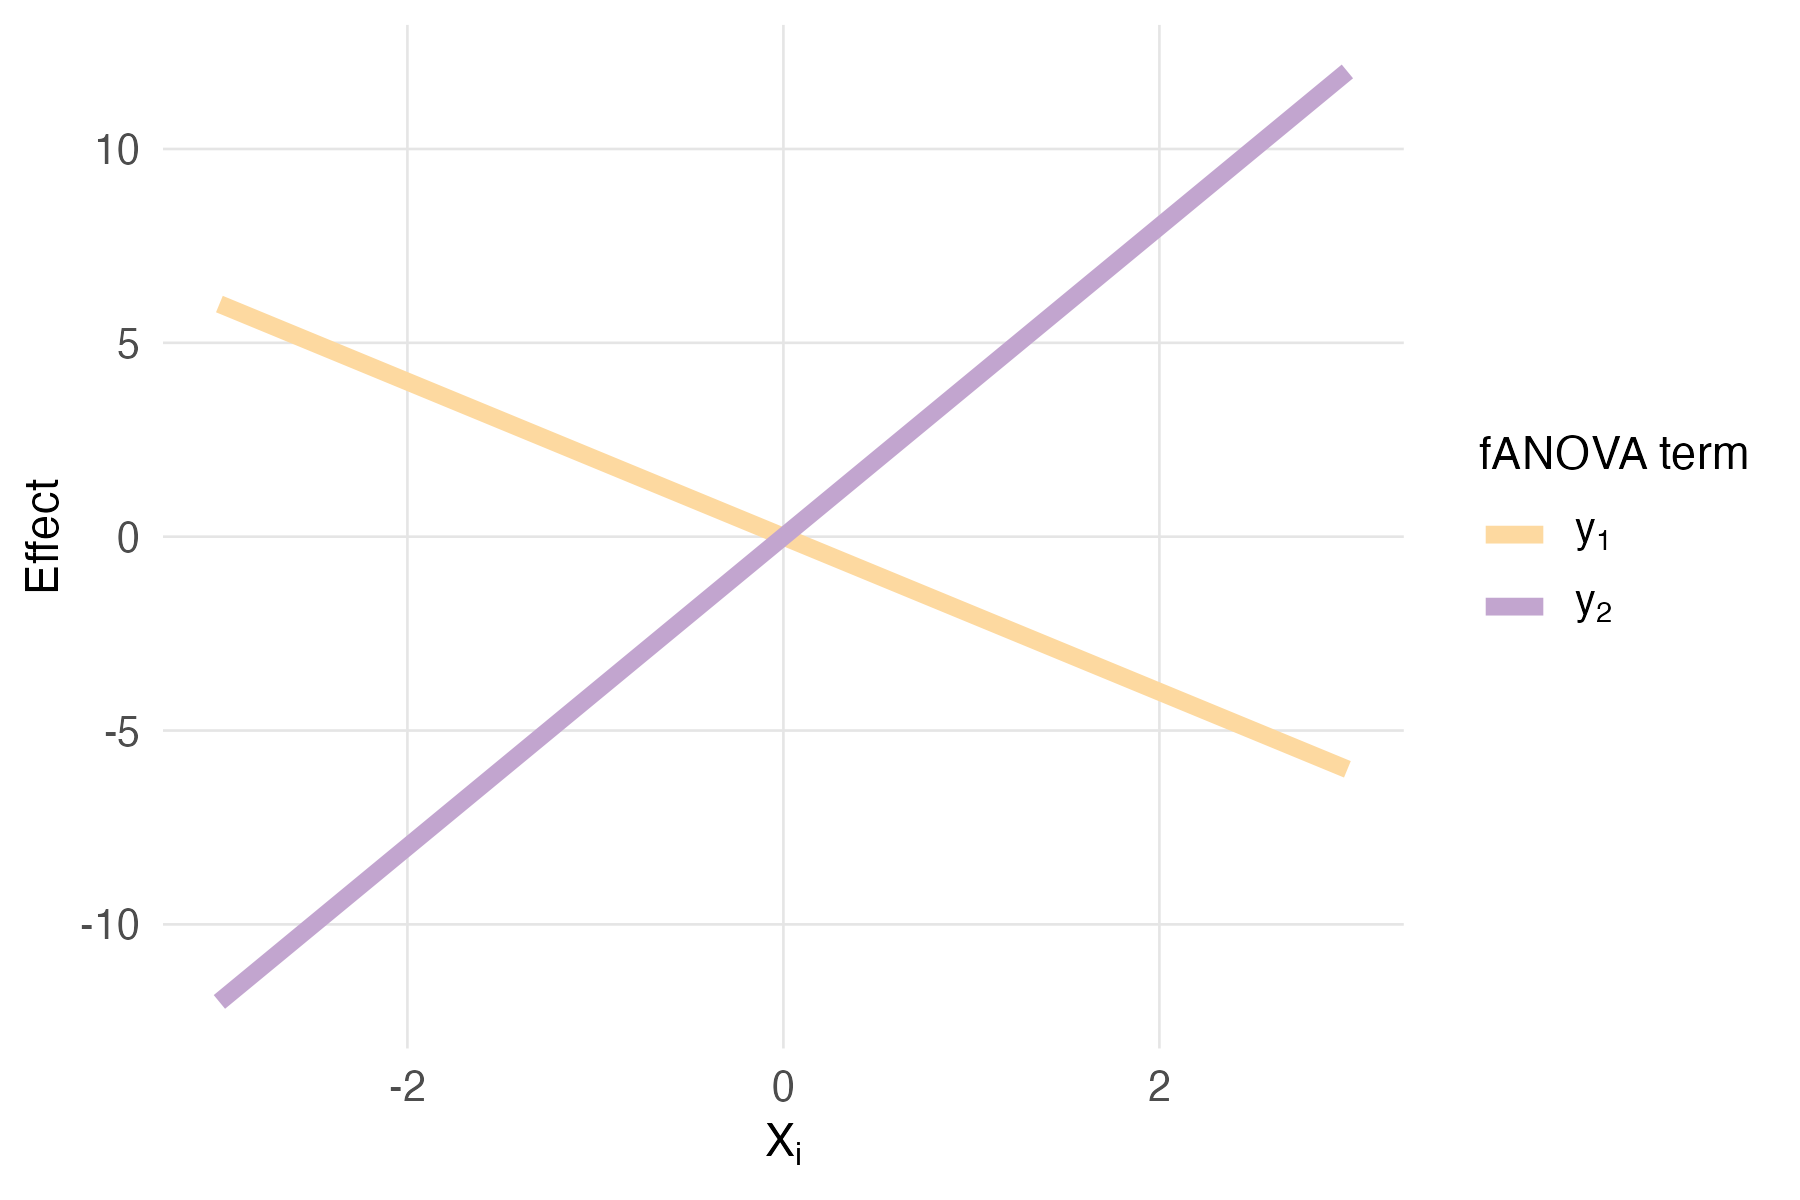
\includegraphics[width=\textwidth]{images/experiment_section/linear_a1m20_a2p40_a11p00_a22p00_a12p00_rhop00_main.png}
        \caption{$a_1 = -2$, $a_2 = 4$}
    \end{subfigure}
    \caption{Main fANOVA components for linear terms with different coefficients. The components are given by: $y_1(x_1) = a_1 x_1$, $y_2(x_2) = a_2 x_2$.}
    \label{fig:linear_main_effects}
\end{figure}



\subsubsection*{Scenario: Quadratic}
Next we consider two-degree polynomials, which contain only quadratic terms. They take the form: $$g_2(x_1, x_2) = a_{11} x_1^2 + a_{22} x_2^2.$$
From \autoref{eq:fanova_components_2D_polynomial} we can derive the fANOVA components for $g_2$:
\begin{align*}
    y_{\emptyset} &= a_{11} + a_{22}, \\
    y_1(x_1) &= a_{11}(x_1^2 - 1), \\
    y_2(x_2) &= a_{22}(x_2^2 - 1).
\end{align*}
In \autoref{fig:quadratic_main_effects}, we vary the coefficients $a_{11}$ and $a_{22}$, while the interaction term is again absent.
Here we deal with two parabolas for the main effect and know that the sign of the coefficients determines their direction, while the magnitudes influence how stretched or compressed they are. The constant fANOVA component $y_{\emptyset}$ is present here, but as it only shifts the decomposition along the y-axis, it does not affect the form of the effect functions, therefore we do not visualize it.

\begin{figure}[htpb]
    \centering
    \begin{subfigure}[t]{0.49\textwidth}
        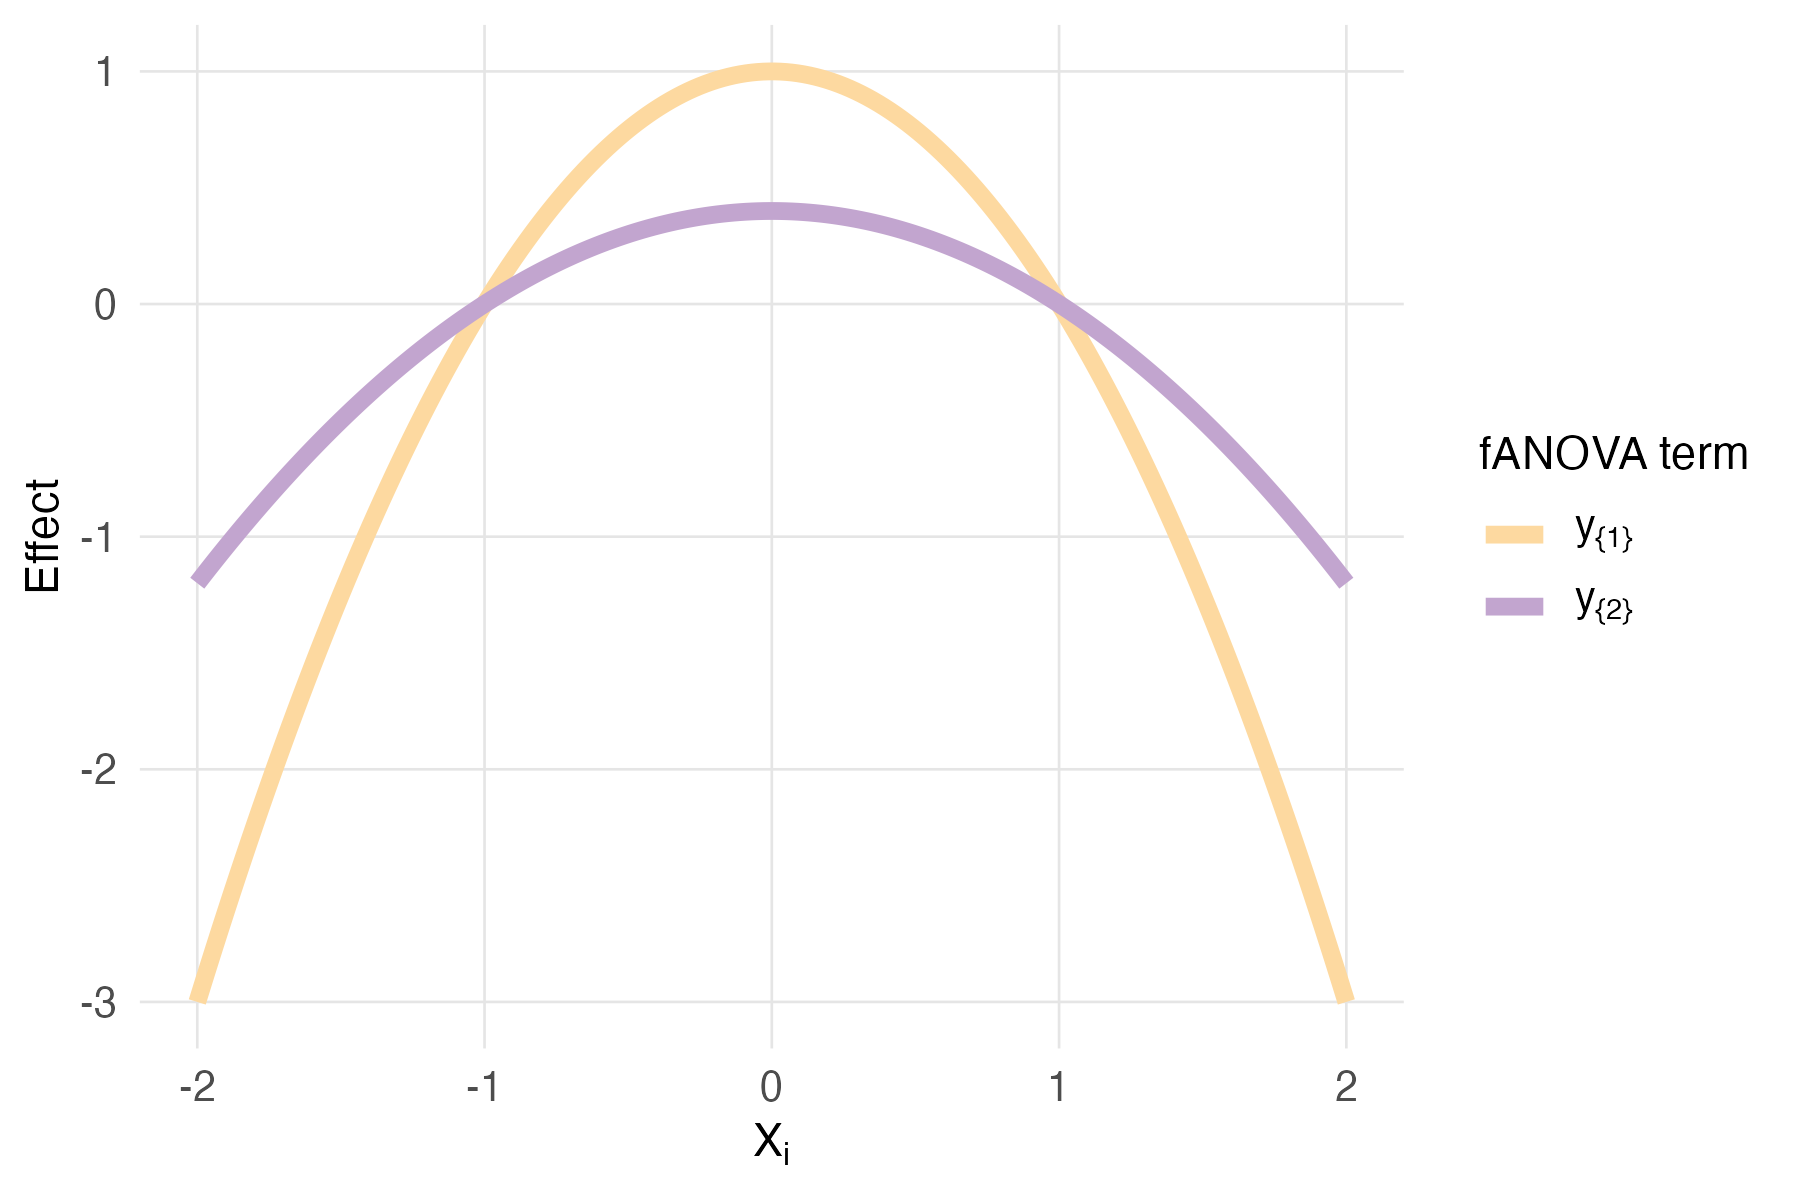
\includegraphics[width=\textwidth]{images/experiment_section/quadratic_a1p00_a2p00_a11m10_a22m04_a12p00_rhop00_main.png}
        \caption{$a_{11} = -1$, $a_{22} = -0.4$}
    \end{subfigure}%
    \hfill
    \begin{subfigure}[t]{0.49\textwidth}
        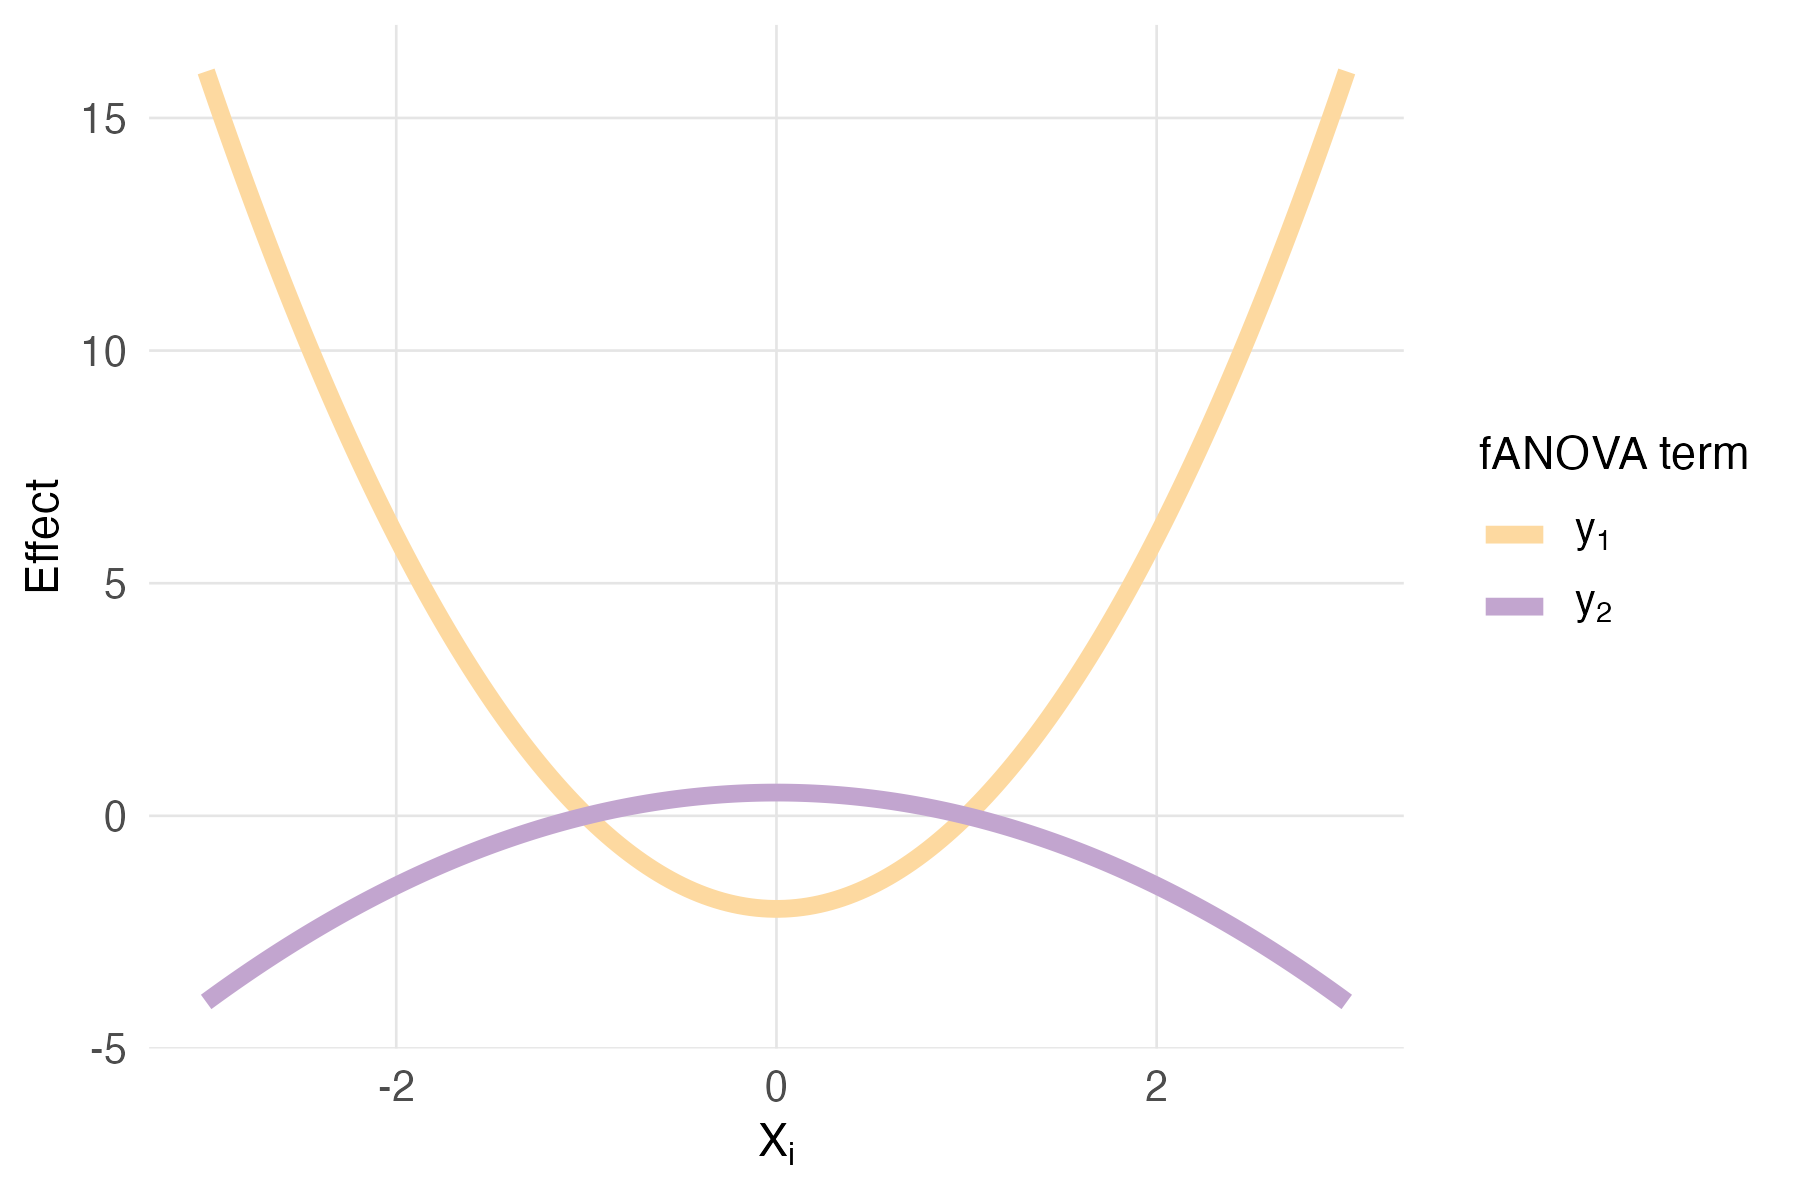
\includegraphics[width=\textwidth]{images/experiment_section/quadratic_a1p00_a2p00_a11p20_a22m05_a12p00_rhop00_main.png}
        \caption{$a_{11} = 2$, $a_{22} = -0.5$}
    \end{subfigure}
    \caption{Main effects for quadratic terms with different coefficients. The fANOVA components are given by: $y_1(x_1) = a_{11}(x_1^2 - 1)$, $y_2(x_2) = a_{22}(x_2^2 - 1)$.}
    \label{fig:quadratic_main_effects}
\end{figure}





\subsubsection*{Scenario: Interaction only}
Next, we consider a model, which solely consists of an interaction term:
$$g_3(x_1, x_2) = a_{12} x_1 x_2.$$
The fANOVA components for $g_3$ are given by:
\begin{align*}
    y_{\emptyset} &= a_{12} \rho, \\
    y_{1}(x_1) &= a_{12} \frac{\rho}{1+ \rho} (x_1^2 - 1), \\
    y_{2}(x_2) &= a_{12} \frac{\rho}{1+ \rho} (x_2^2 - 1), \\
    y_{12}(x_1,x_2) 
&= -a_{12}\!\left(
    \frac{\rho(x_1^2+x_2^2)}{1+\rho^2} 
    - x_1 x_2 
    + \frac{\rho(\rho^2-1)}{1+\rho^2}
   \right).
\end{align*}
What is interesting to see is that the main effects are present, due to the dependence between variable, even though there are no isolated main effects in $g_3$.
The main effects $y_1$ and $y_2$, as well as the interaction term $y_{12}$, are influenced by $\rho$ and $a_{12}$.
In our example we keep $a_{12} = 2$ fixed and show the interaction effect as a contour plot for varying $\rho$ with the corresponding main effects next to it \autoref{fig:interaction_combined}. For every case of $\rho$ and $a_{12}$, the main effects have the same form, therefore they overlap.
\begin{figure}[htpb]
    \centering
    % ----- Row 1 -----
    \begin{subfigure}[t]{0.49\textwidth}
        \centering
        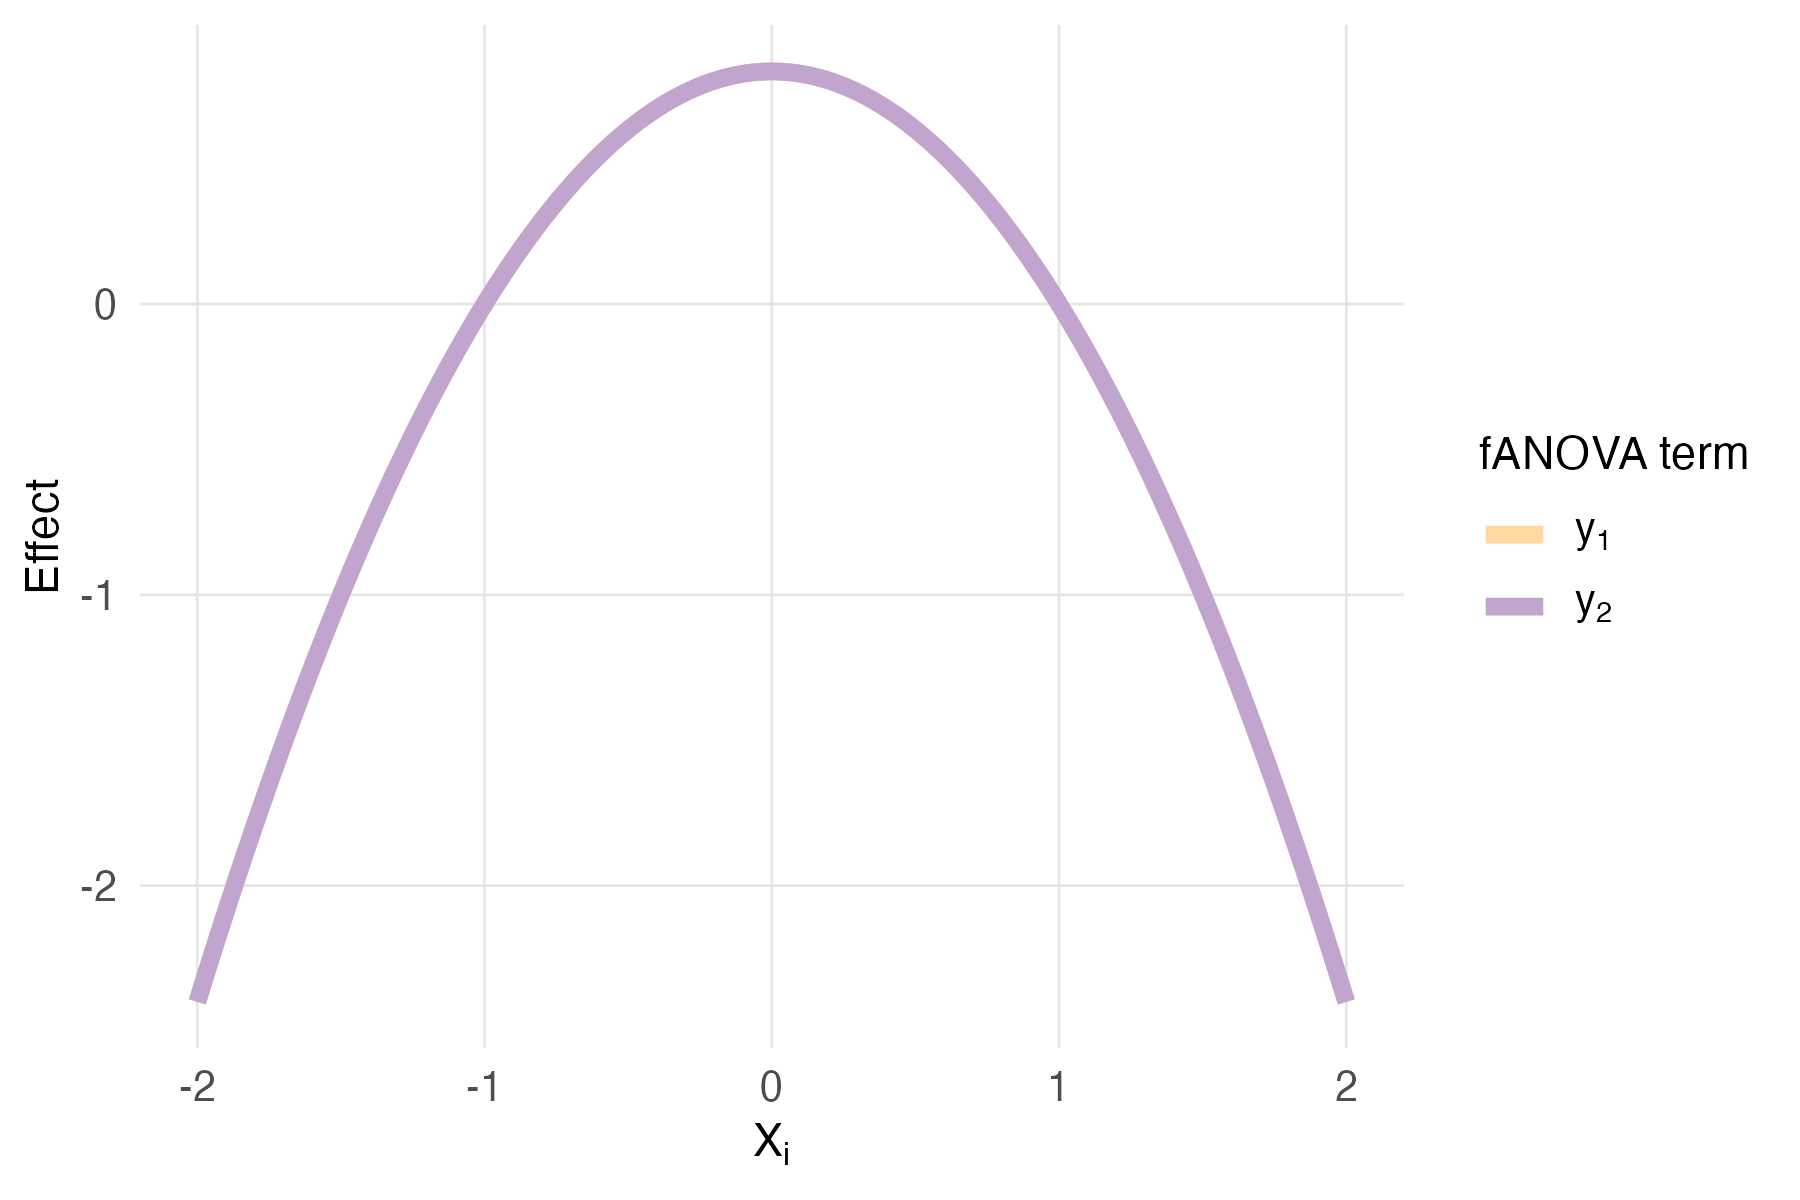
\includegraphics[width=\textwidth]{images/experiment_section/interaction_a1p00_a2p00_a11p00_a22p00_a12p20_rhom05_main.png}
        \caption{Main effects for $\rho = -0.5$}
    \end{subfigure}%
    \hfill
    \begin{subfigure}[t]{0.49\textwidth}
        \centering
        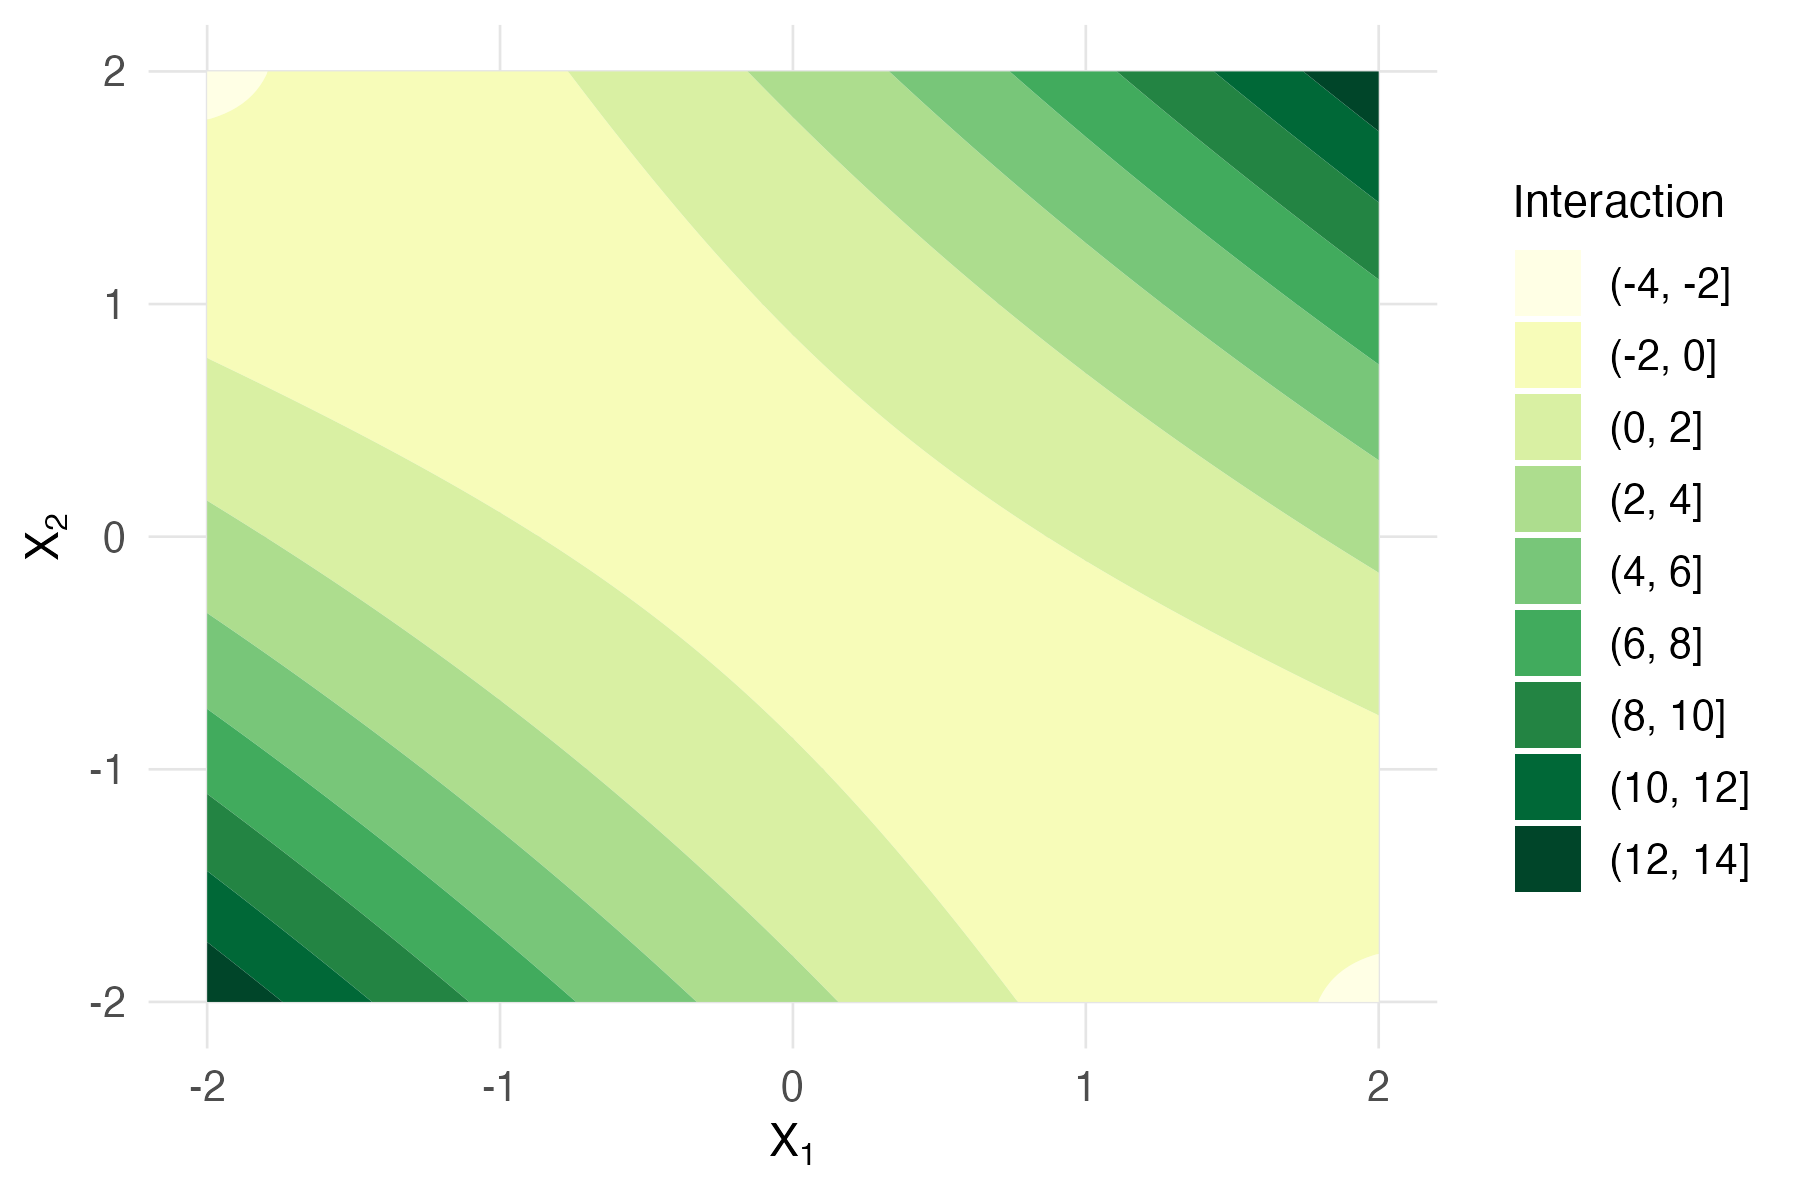
\includegraphics[width=\textwidth]{images/experiment_section/interaction_a1p00_a2p00_a11p00_a22p00_a12p20_rhom05_interaction.png}
        \caption{Interaction contour for $\rho = -0.5$}
    \end{subfigure}

    \vspace{0.5em}
    % ----- Row 2 -----
    \begin{subfigure}[t]{0.49\textwidth}
        \centering
        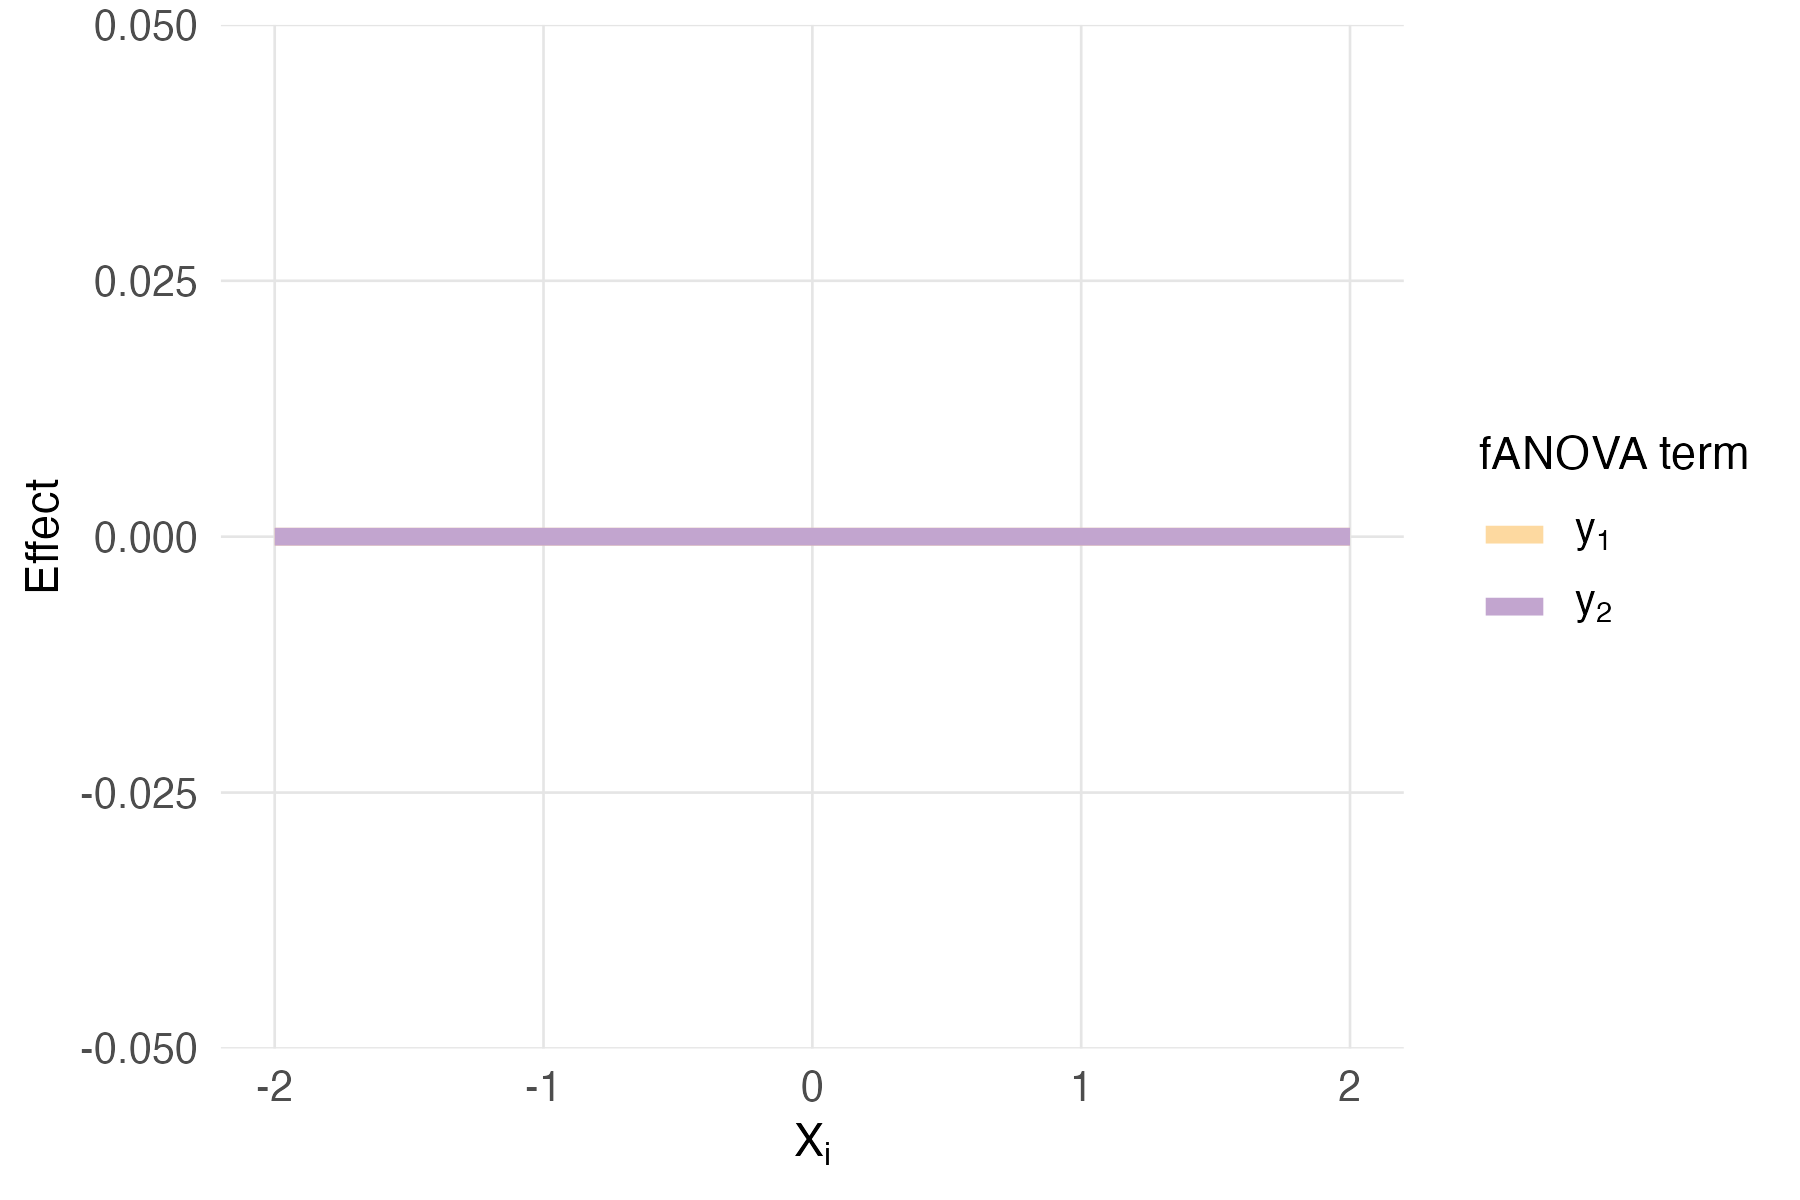
\includegraphics[width=\textwidth]{images/experiment_section/interaction_a1p00_a2p00_a11p00_a22p00_a12p20_rhop00_main.png}
        \caption{Main effects for $\rho = 0$}
    \end{subfigure}%
    \hfill
    \begin{subfigure}[t]{0.49\textwidth}
        \centering
        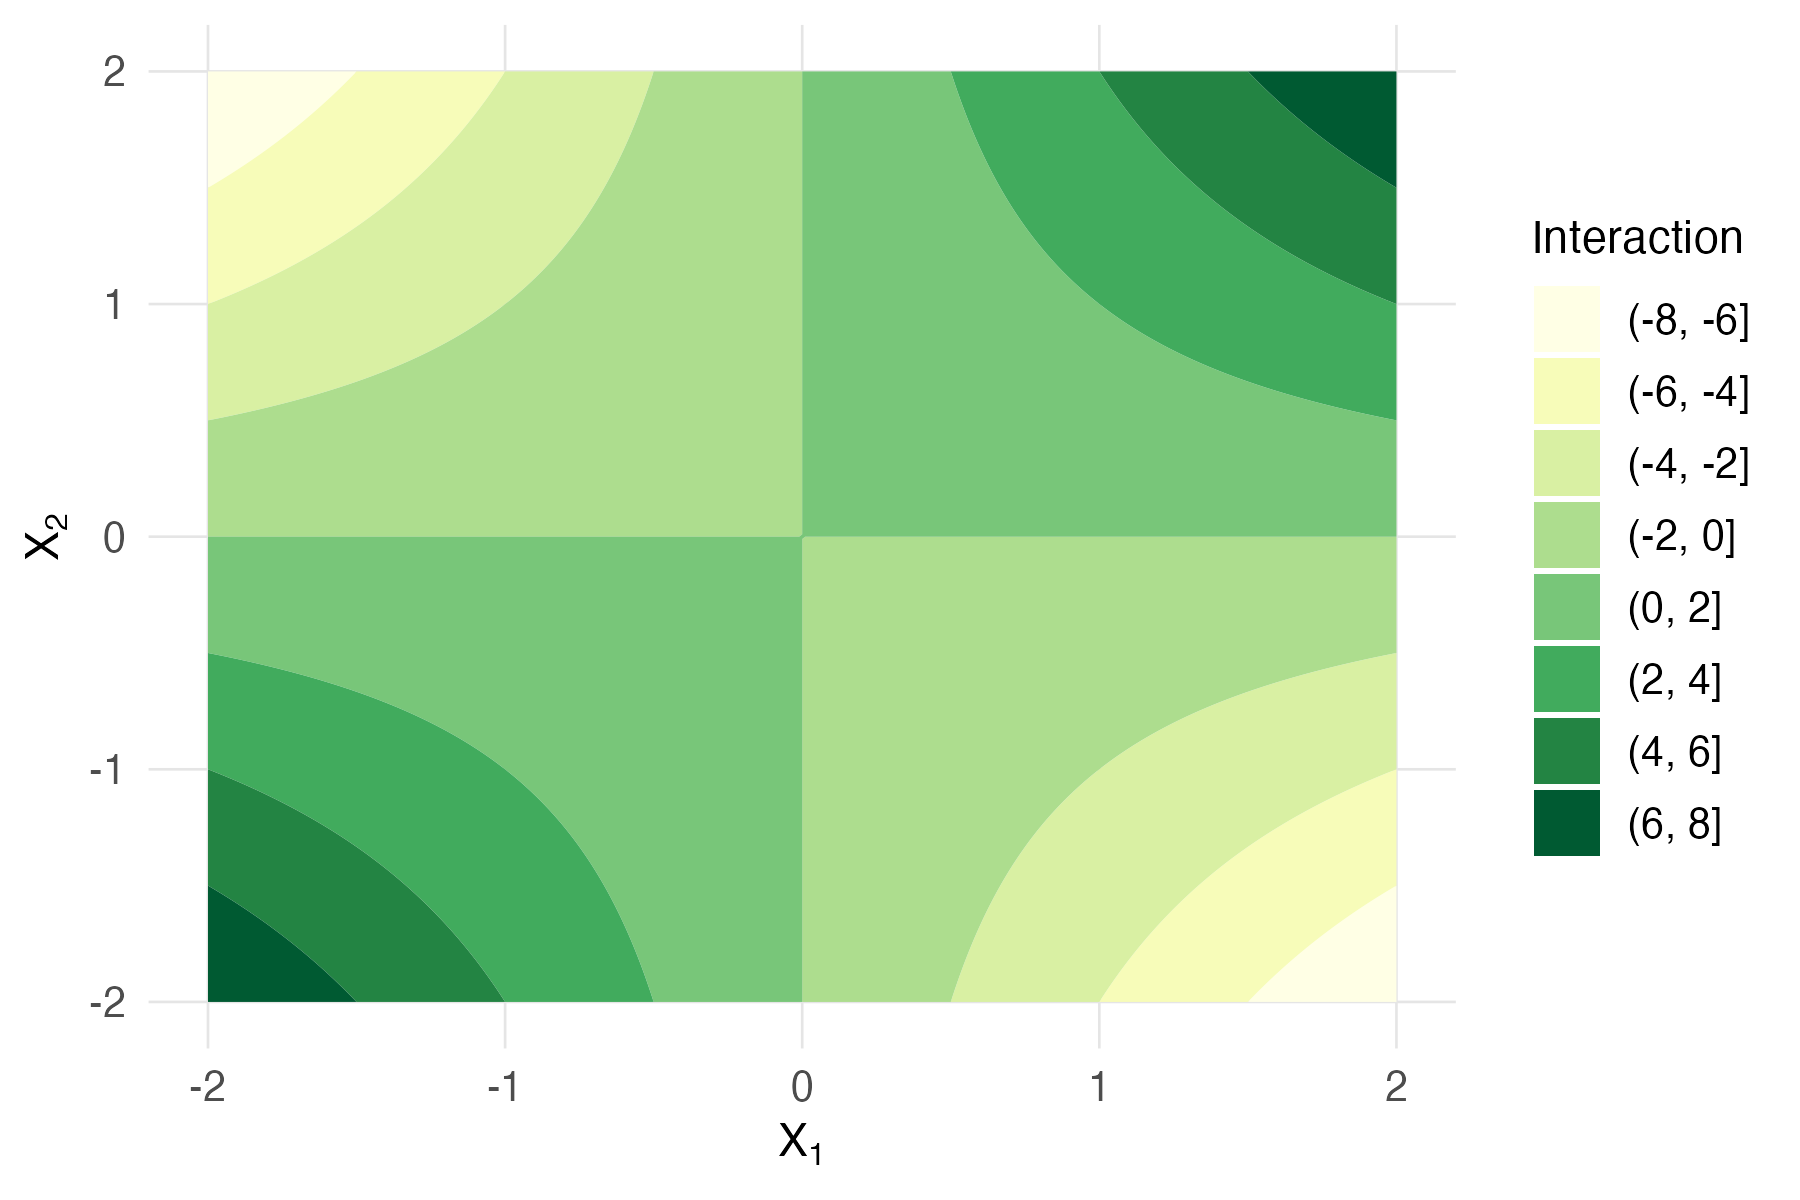
\includegraphics[width=\textwidth]{images/experiment_section/interaction_a1p00_a2p00_a11p00_a22p00_a12p20_rhop00_interaction.png}
        \caption{Interaction contour for $\rho = 0$}
    \end{subfigure}

    \vspace{0.5em}
    % ----- Row 3 -----
    \begin{subfigure}[t]{0.49\textwidth}
        \centering
        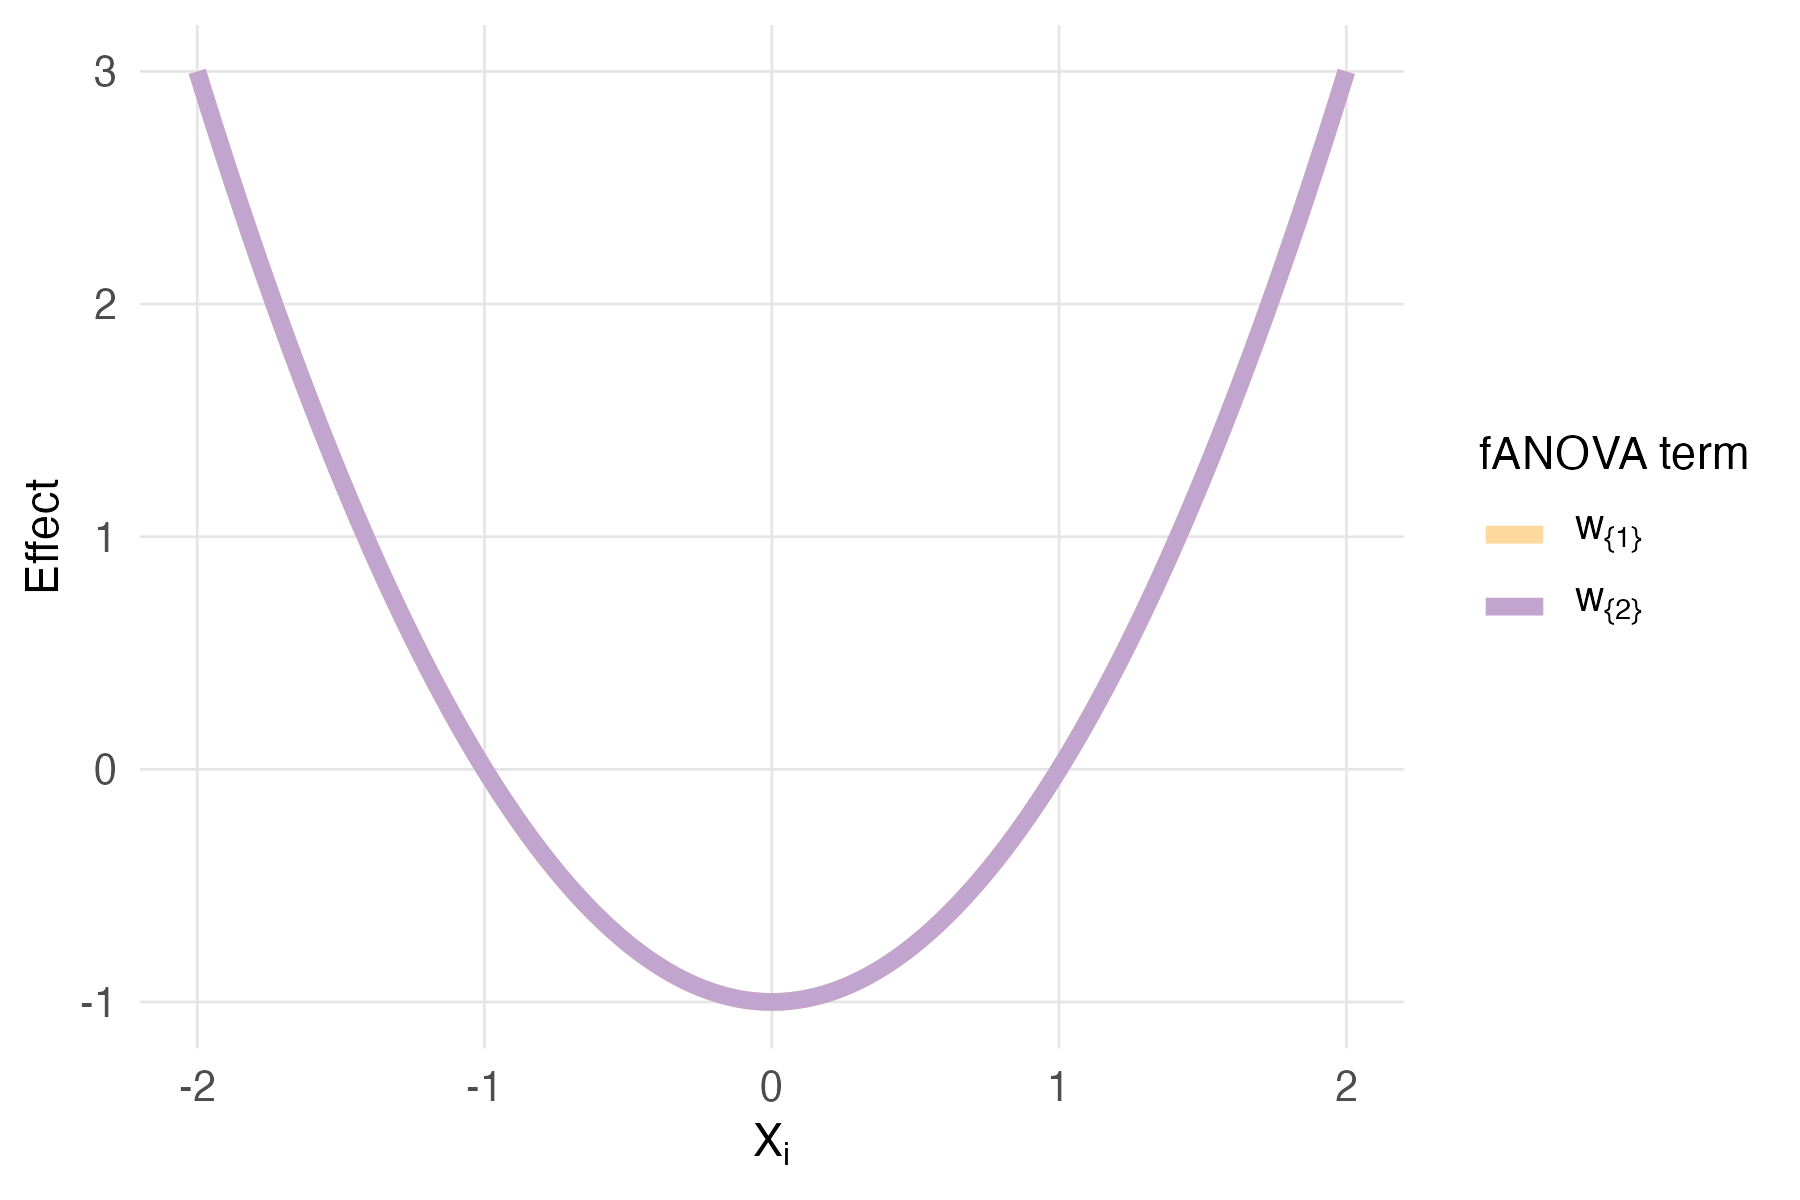
\includegraphics[width=\textwidth]{images/experiment_section/interaction_a1p00_a2p00_a11p00_a22p00_a12p20_rhop10_main.png}
        \caption{Main effects for $\rho = 1$}
    \end{subfigure}%
    \hfill
    \begin{subfigure}[t]{0.49\textwidth}
        \centering
        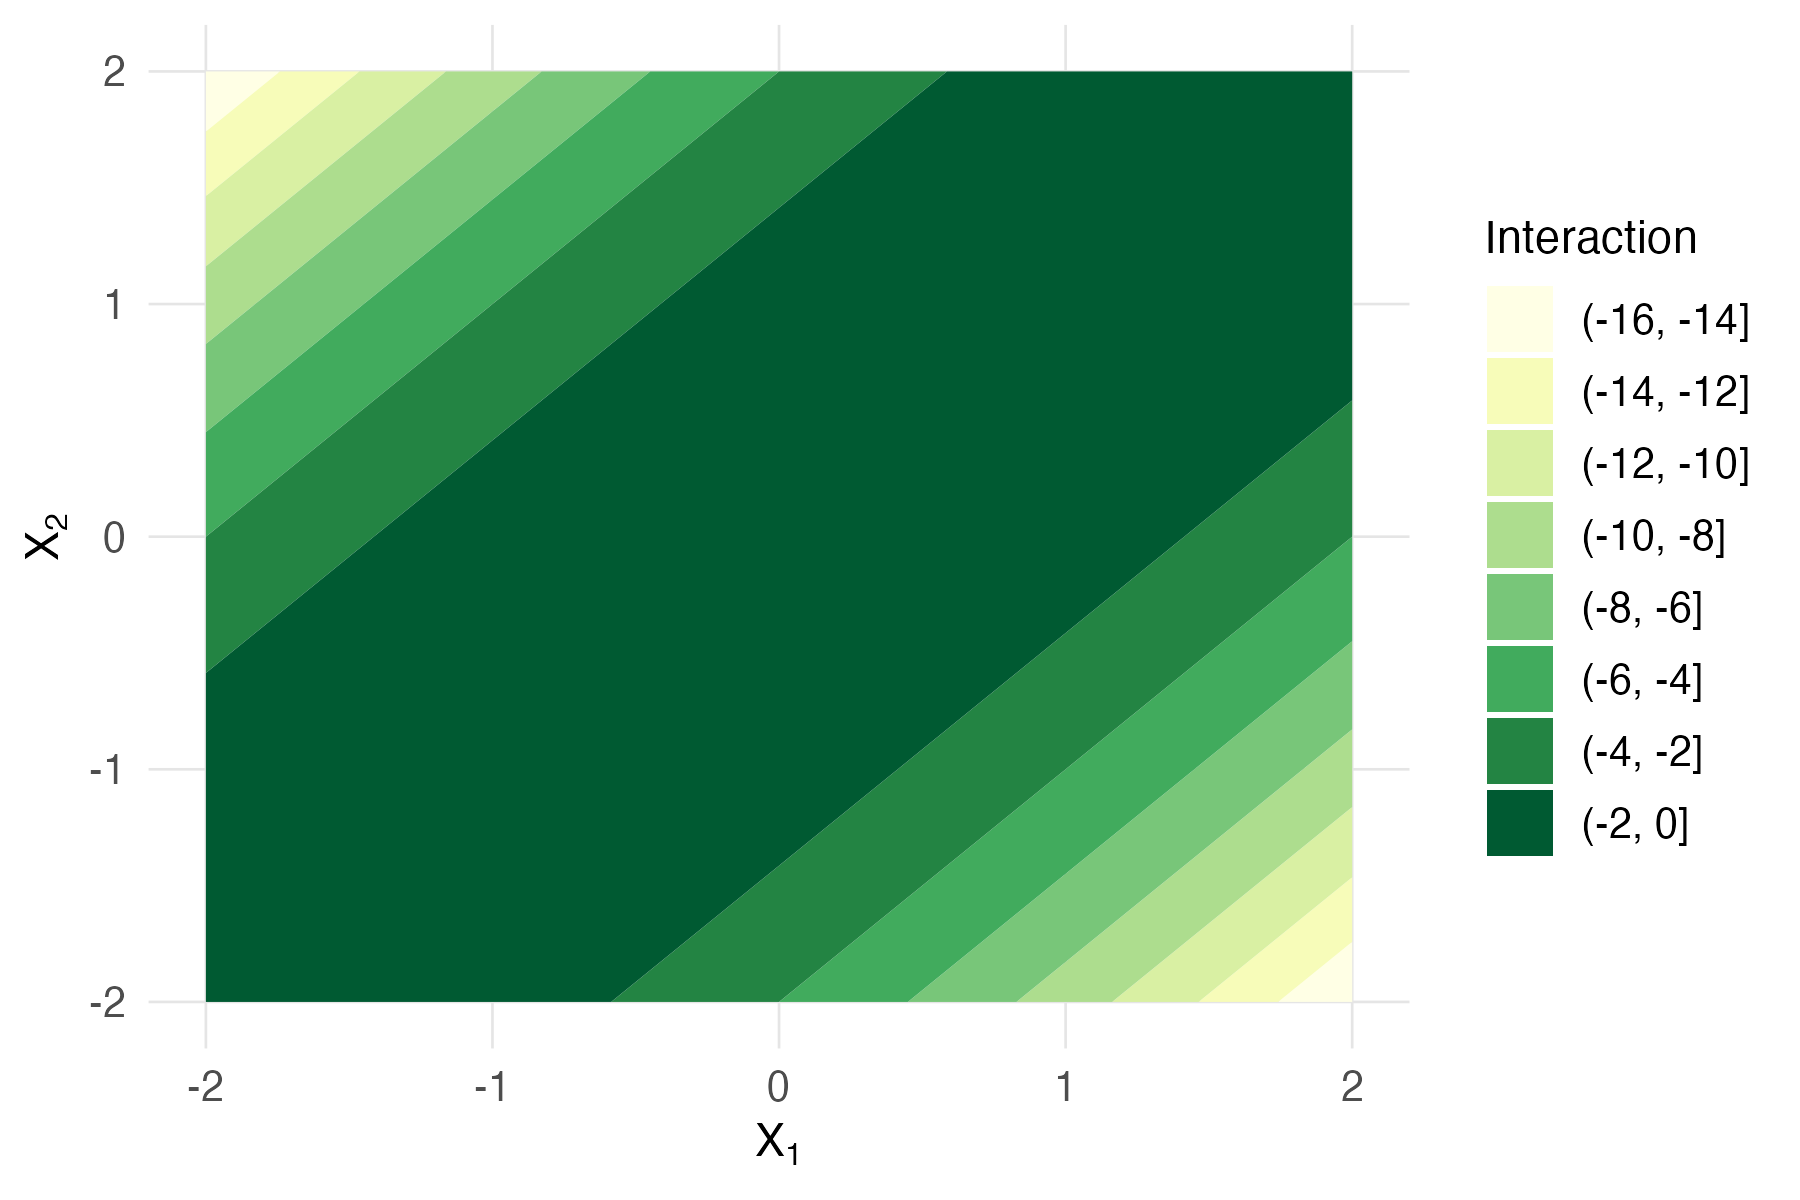
\includegraphics[width=\textwidth]{images/experiment_section/interaction_a1p00_a2p00_a11p00_a22p00_a12p20_rhop10_interaction.png}
        \caption{Interaction contour for $\rho = 1$}
    \end{subfigure}

    \caption{Main effects (left column) and interaction contour plots (right column) for different values of $\rho$. The effects are given by $y_{1}(x_1) = a_{12} \frac{\rho}{1+ \rho} (x_1^2 - 1)$,
    $y_{2}(x_2) = a_{12} \frac{\rho}{1+ \rho} (x_2^2 - 1)$,
    $y_{12}(x_1,x_2) = -a_{12}\!\left(\frac{\rho(x_1^2+x_2^2)}{1+\rho^2} - x_1 x_2 + \frac{\rho(\rho^2-1)}{1+\rho^2}\right)$.}
    \label{fig:interaction_combined}
\end{figure}



\subsubsection*{Scenario: Mixed, only main}
Following, we study the main effects of two-degree polynomials, which allow for effects of linear and quadratic nature:
\[
g_4(x_1, x_2) = a_1 x_1 + a_2 x_2 + a_{11} x_1^2 + a_{22} x_2^2.
\]
The fANOVA components for $g_4$ are given by:
\begin{align*}
    y_{\emptyset} &= a_{11} + a_{22}, \\
    y_1(x_1) &= a_1 x_1 + a_{11}(x_1^2 - 1), \\
    y_2(x_2) &= a_2 x_2 + a_{22}(x_2^2 - 1).
\end{align*}
In \autoref{fig:mixed_main_effects}, we vary the coefficients $a_1$, $a_2$, $a_{11}$, and $a_{22}$, while the interaction term is again absent.
The shape of the parabolas in the upper left panel is representative of cases, where the coefficients of the linear terms $a_1$ and $a_2$ have the same sign and the ones of the quadratic terms $a_{11}$ and $a_{22}$ have the same sign.
The coefficients of the quadratic terms $a_{11}$ and $a_{22}$ determine whether the parabola is facing downwards or upwards; when they are both negative the parabola is open downwards and when they are both positive the parabola is upwards open. Alongside the quadratic coefficients, the linear ones $a_1$ and $a_2$ influence how stretched or compressed the parabola is.\par
The upper right plot and the lower left plot show typical behaviour for cases where the quadratic coefficients have different signs. In such cases we get parabolas that are open in opposite directions.
% The only systematic difference between the upper right and lower left is that within variable sign-difference is only true for one variable, either $X_1$ or $X_2$ in the lower left plot.\par
Lastly, in the lower right we have cases where the signs of the linear coefficient $a_i$ is different than of the quadratic coefficient $a_{ii}$ within the same Variable $X_i$, but the signs of the quadratic coefficients are the same between variables (so $a_{ii}$ and $a_{jj}$ have the same sign). Here we have a symmetric pattern, where the parabolas are open in the same direction and otherwise may look different.

% The upper right plot is representative of cases where we have within-variable sign difference and a symmetric between variable sign-difference, for example we look at cases such as $a_1 = -2, a_{11} = 1, a_2 = 2, a_{22} = -1$ or $a_1 = 2, a_{11} = -1, a_2 = -2, a_{22} = 1$. Here again, whether the parabola for a variable is facing upwards or downwards is determined by the sign of the quadratic coefficient.
% In the lower left we represent cases in which within-variable sign difference is only true for one variable, either $X_1$ or $X_2$, and the quadratic coefficients are sign-different. Then we get parabolas that are open in opposite directions.\par
% where we have 1. the same sign \textit{within} a variable and where we have 2. different signs \textit{within} a variable, but they are different in the same way for both variables. 1. includes sets of coefficients like
% $a1 = -2, a11 = -1, a2 = -2, a22 = -1$. 2. includes sets of coefficients like $a1 = 2, a11 = -1, a2 = 2, a22 = -1$ or $a1 = -2, a11 = -1, a2 = -2, a22 = 1$.
\begin{figure}[htpb]
    \centering
    % --- Row 1 ---
    \begin{subfigure}[t]{0.49\textwidth}
        \centering
        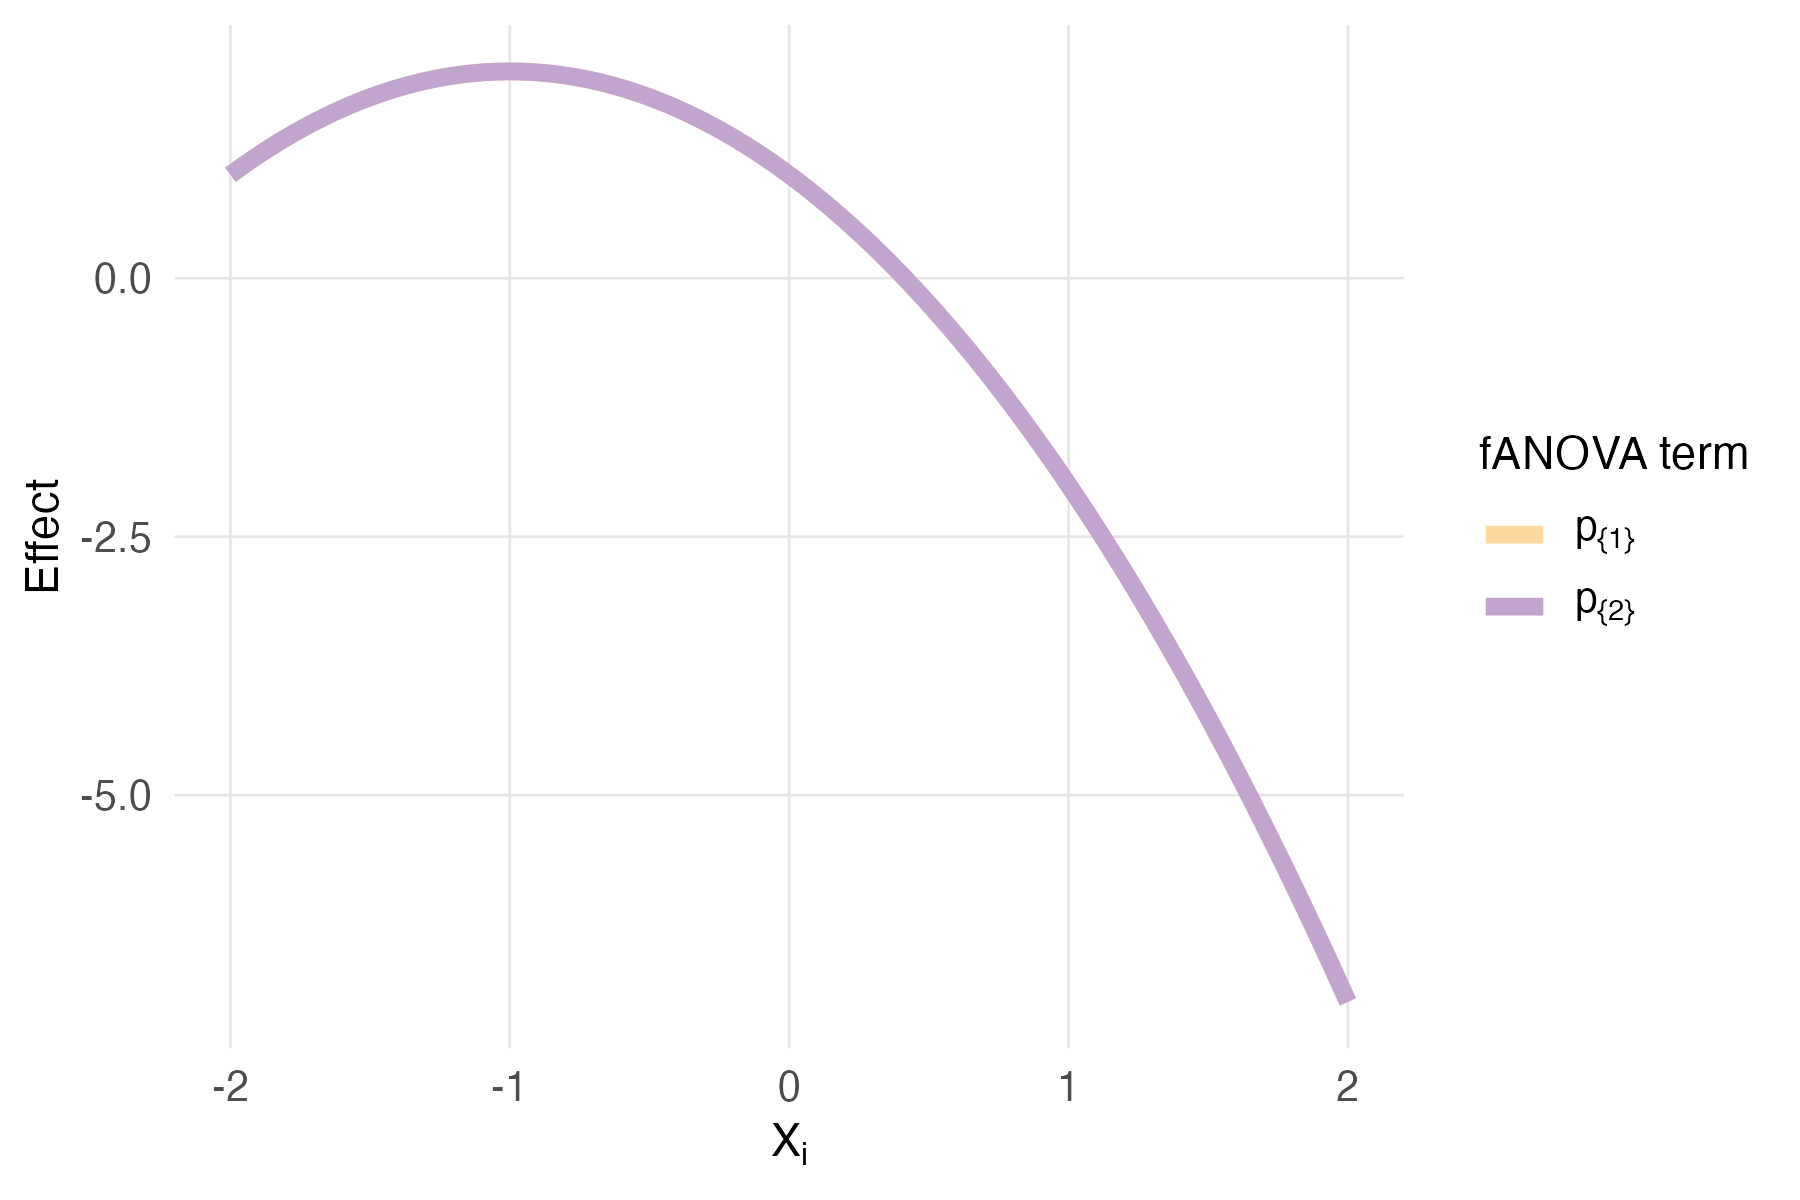
\includegraphics[width=\textwidth]{images/experiment_section/mixed_a1m20_a2m20_a11m10_a22m10_a12p00_rhop00_main.png}
        \caption{$a_1=-2,\, a_2=-2,\, a_{11}=-1,\, a_{22}=-1$}
        \label{fig:mixed_rho_0_panel1}
    \end{subfigure}%
    \hfill
    \begin{subfigure}[t]{0.49\textwidth}
        \centering
        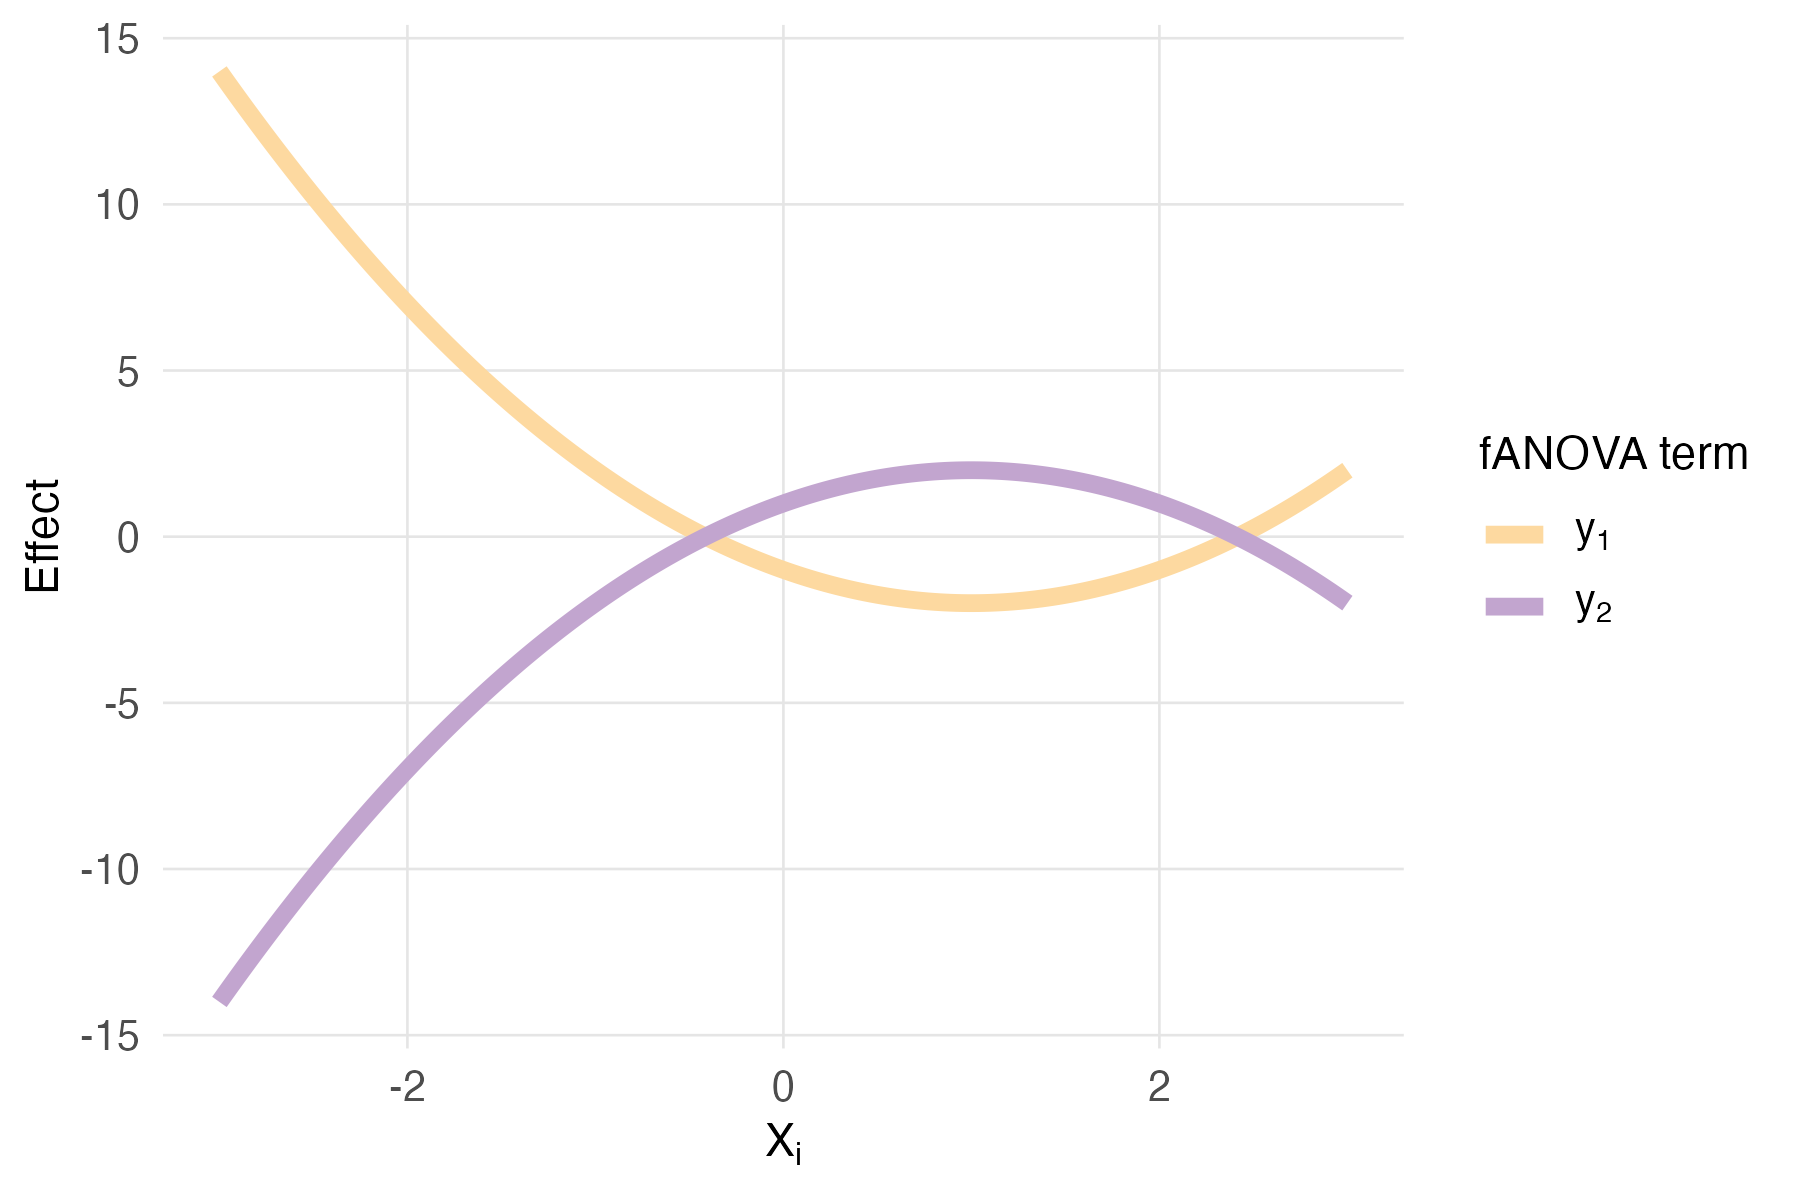
\includegraphics[width=\textwidth]{images/experiment_section/mixed_a1m20_a2p20_a11p10_a22m10_a12p00_rhop00_main.png}
        \caption{$a_1=-2,\, a_2=2,\, a_{11}=1,\, a_{22}=-1$}
        \label{fig:mixed_rho_0_panel2}
    \end{subfigure}

    % --- Row 2 ---
    \begin{subfigure}[t]{0.49\textwidth}
        \centering
        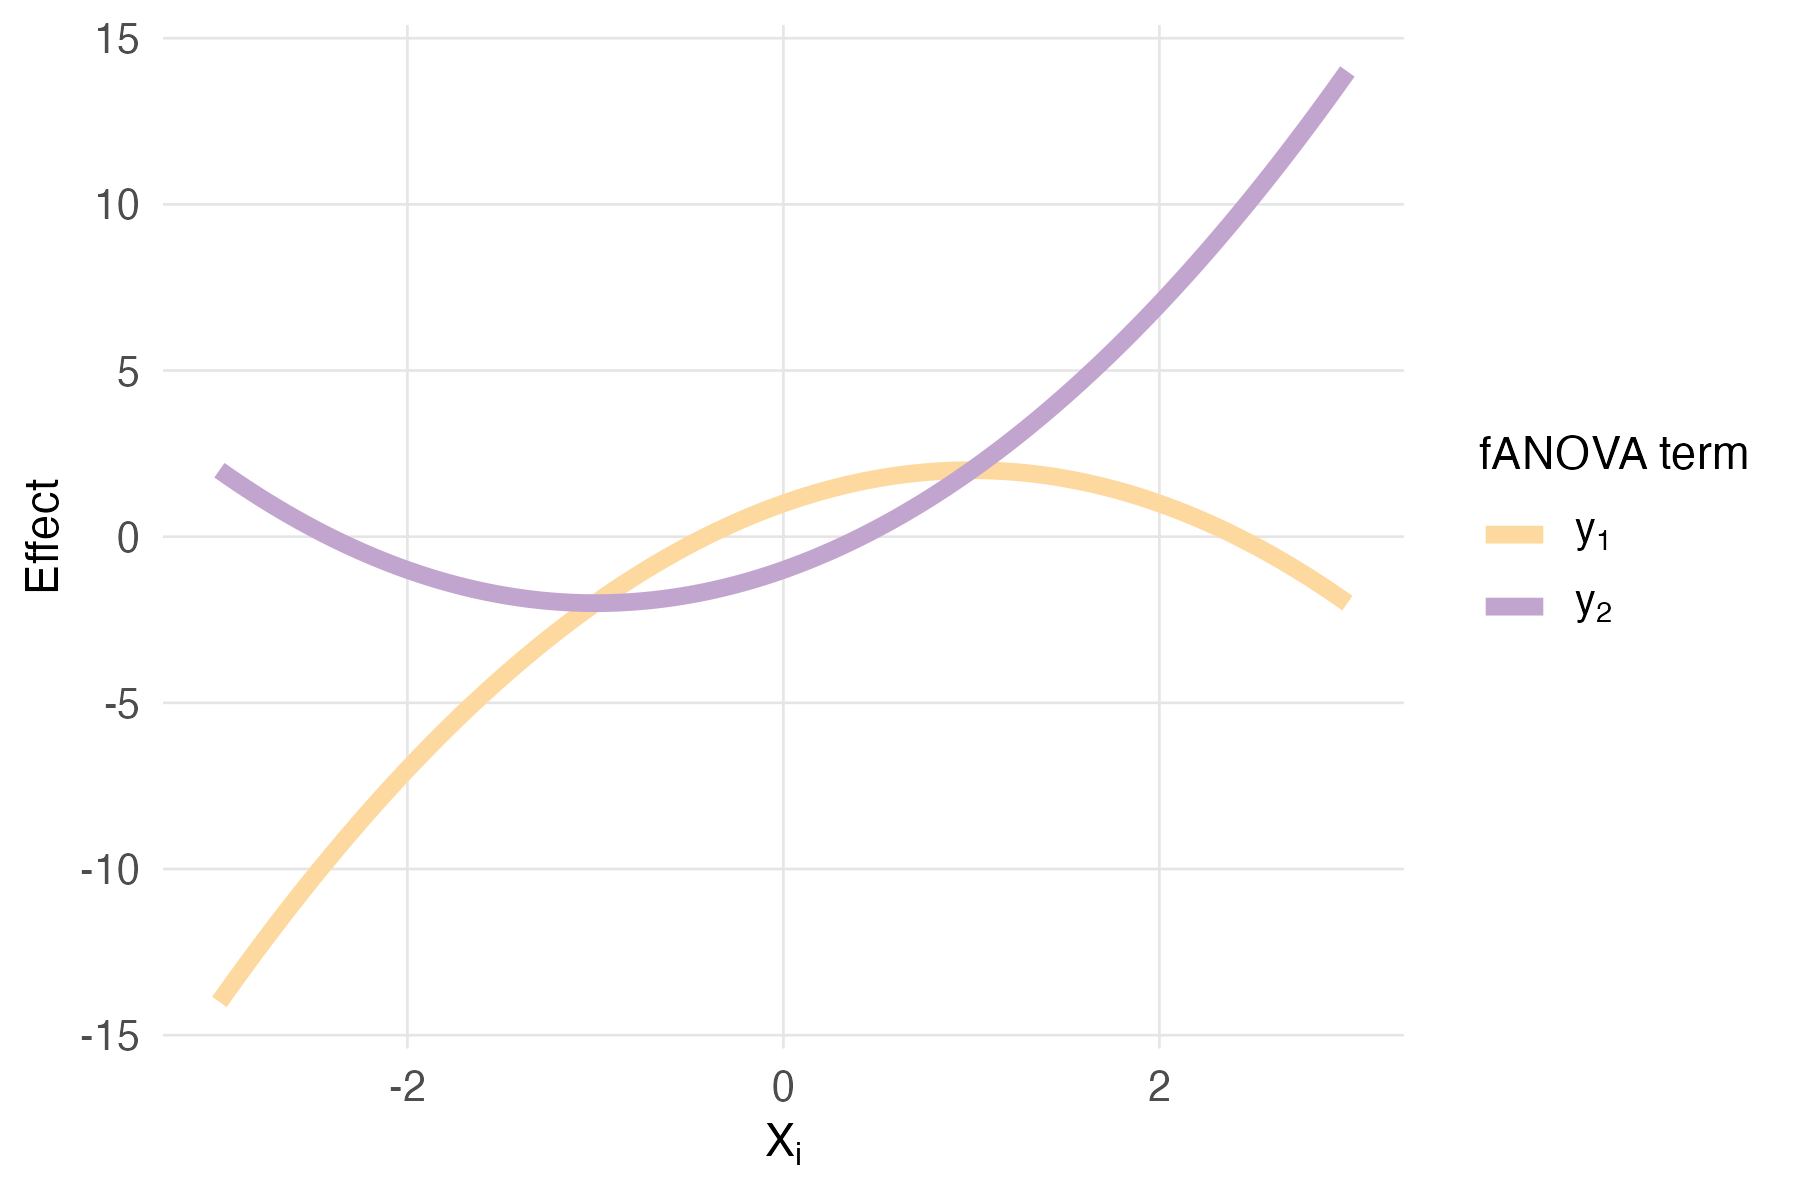
\includegraphics[width=\textwidth]{images/experiment_section/mixed_a1p20_a2p20_a11m10_a22p10_a12p00_rhop00_main.png}
        \caption{$a_1=2,\, a_2=2,\, a_{11}=-1,\, a_{22}=1$}
        \label{fig:mixed_rho_0_panel3}
    \end{subfigure}%
    \hfill
    \begin{subfigure}[t]{0.49\textwidth}
        \centering
        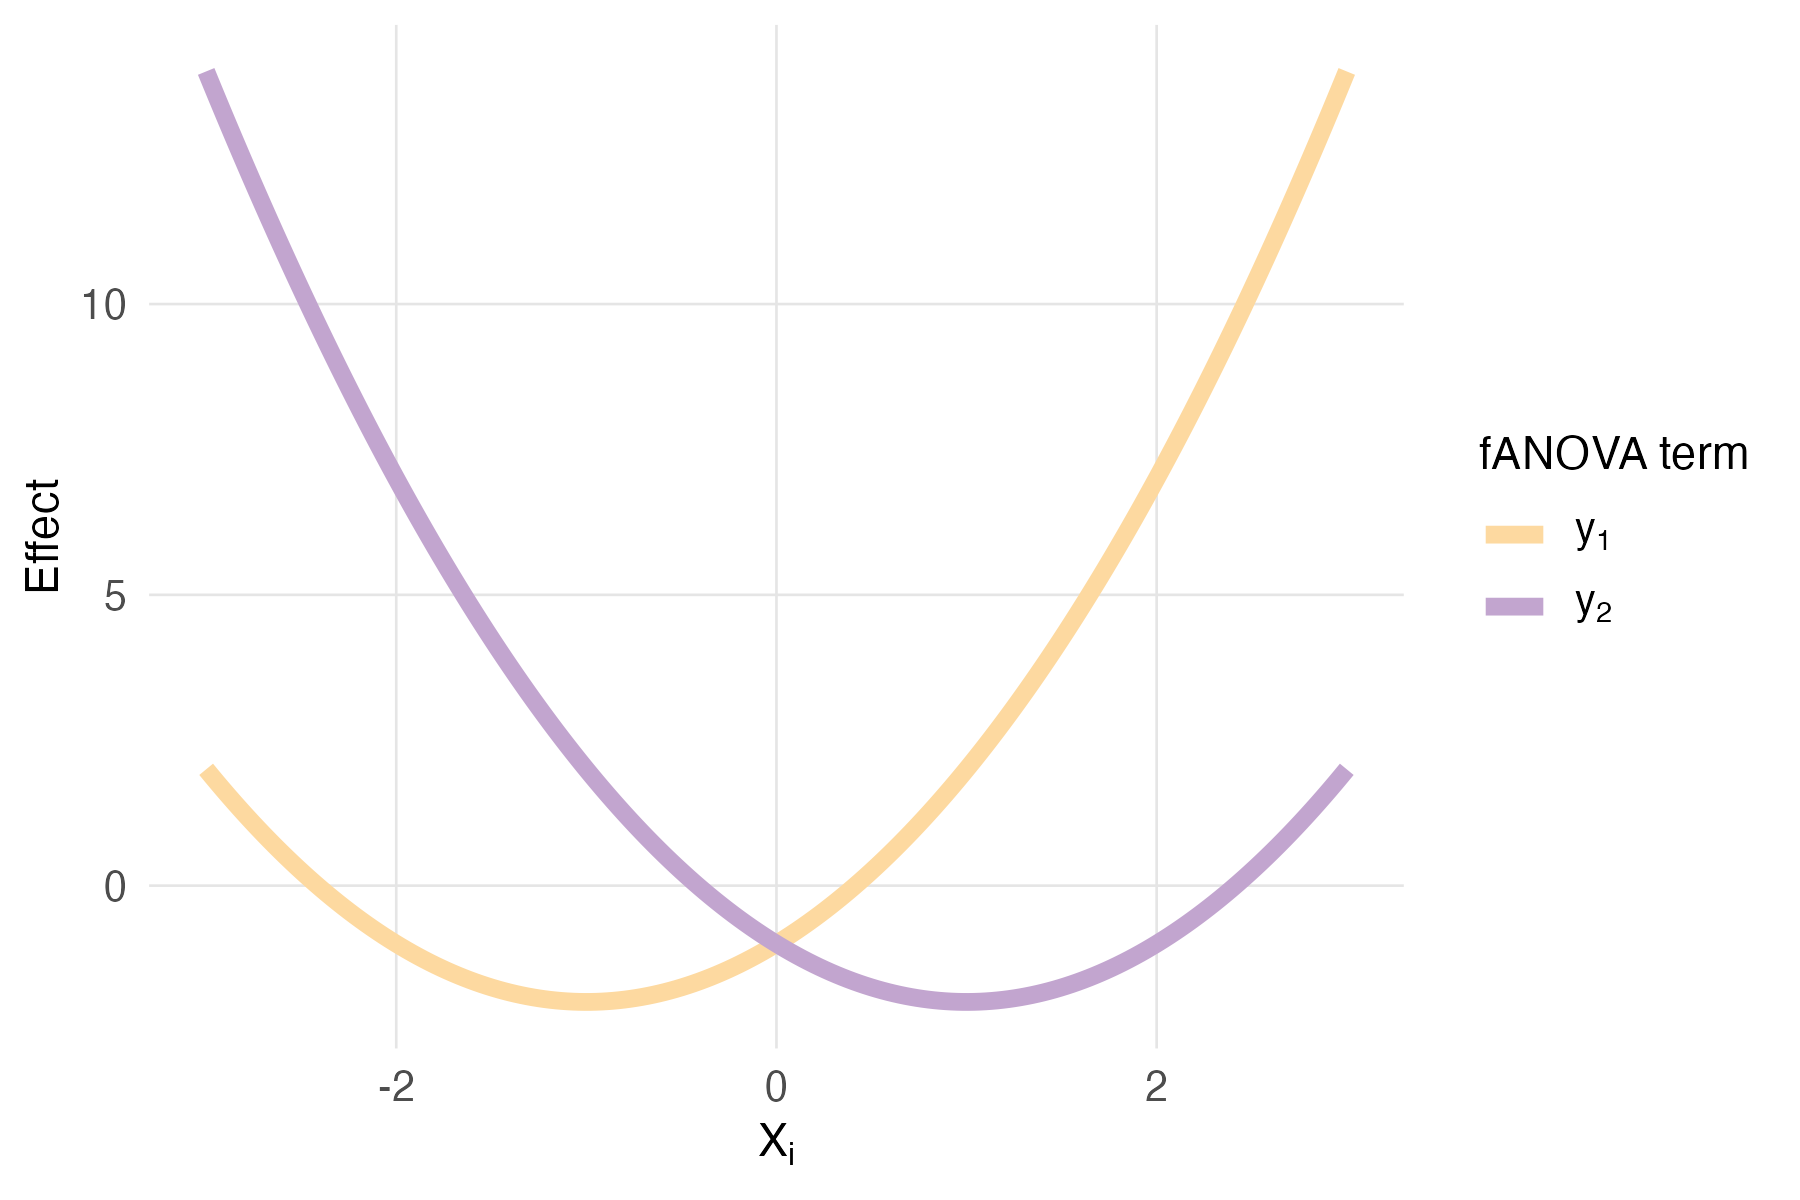
\includegraphics[width=\textwidth]{images/experiment_section/mixed_a1p20_a2m20_a11p10_a22p10_a12p00_rhop00_main.png}
        \caption{$a_1=2,\, a_2=-2,\, a_{11}=1,\, a_{22}=1$}
        \label{fig:mixed_rho_0_panel4}
    \end{subfigure}

    \caption{Main effects for different coefficient combinations of mixed main effects. The commponents are given by: $y_1(x_1) = a_1 x_1 + a_{11}(x_1^2 - 1)$, $y_2(x_2) = a_2 x_2 + a_{22}(x_2^2 - 1)$.}
    \label{fig:mixed_main_effects}
\end{figure}




\subsubsection*{Scenario: All}
Finally full example, including all main and interaction effects:
$$g_5(x_1, x_2) = a_1 x_1 + a_2 x_2 + a_{11} x_1^2 + a_{22} x_2^2 + a_{12} x_1 x_2.$$
Now the fANOVA components are given by \autoref{eq:fanova_components_2D_polynomial}, where $a_0 = 0$.
We can vary the coefficients as well as $\rho$.\par
We recognize the patterns from previous examples which had less parameters to vary.
Whether the parabolas are facing upwards or downwards is determined by the sign of the quadratic coefficients.
Whether they are facing in the same direction is determined by between variable sign-difference of the quadratic coefficients.
Under presence of an interaction term,
the direction in which the main effects are facing is also influenced by $\rho$.
The linear coefficients only have an influence on how stretched or compressed the parabolas are.
The interaction term is influenced by $\rho$ and $a_{12}$.\par
\begin{figure}[htpb]
    \centering

    % -------- Pair 1 --------
    \begin{subfigure}[t]{\textwidth}
        \centering
        \begin{minipage}[t]{0.49\textwidth}
            \centering
            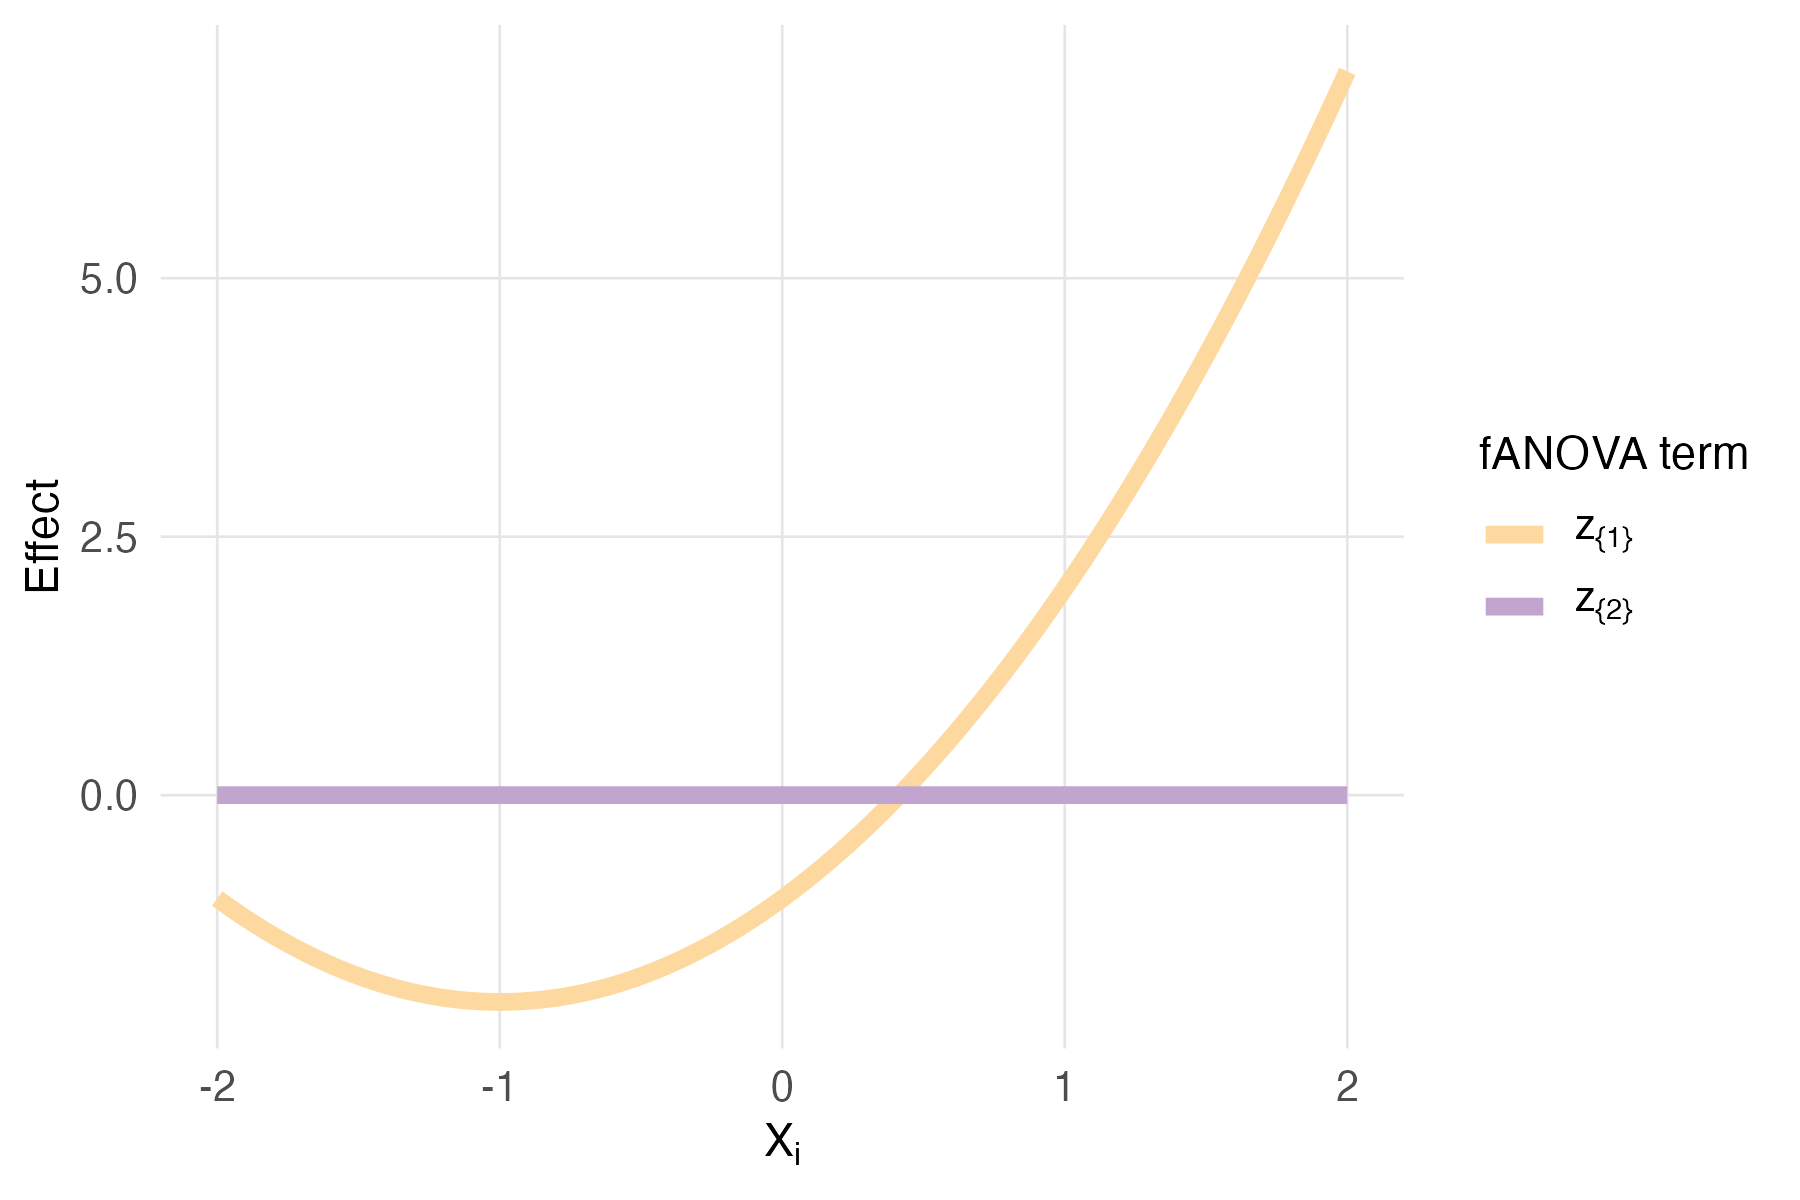
\includegraphics[width=\textwidth]{images/experiment_section/full_a1p20_a2p00_a11p10_a22p00_a12p05_rhop00_main.png}
        \end{minipage}%
        \hfill
        \begin{minipage}[t]{0.49\textwidth}
            \centering
            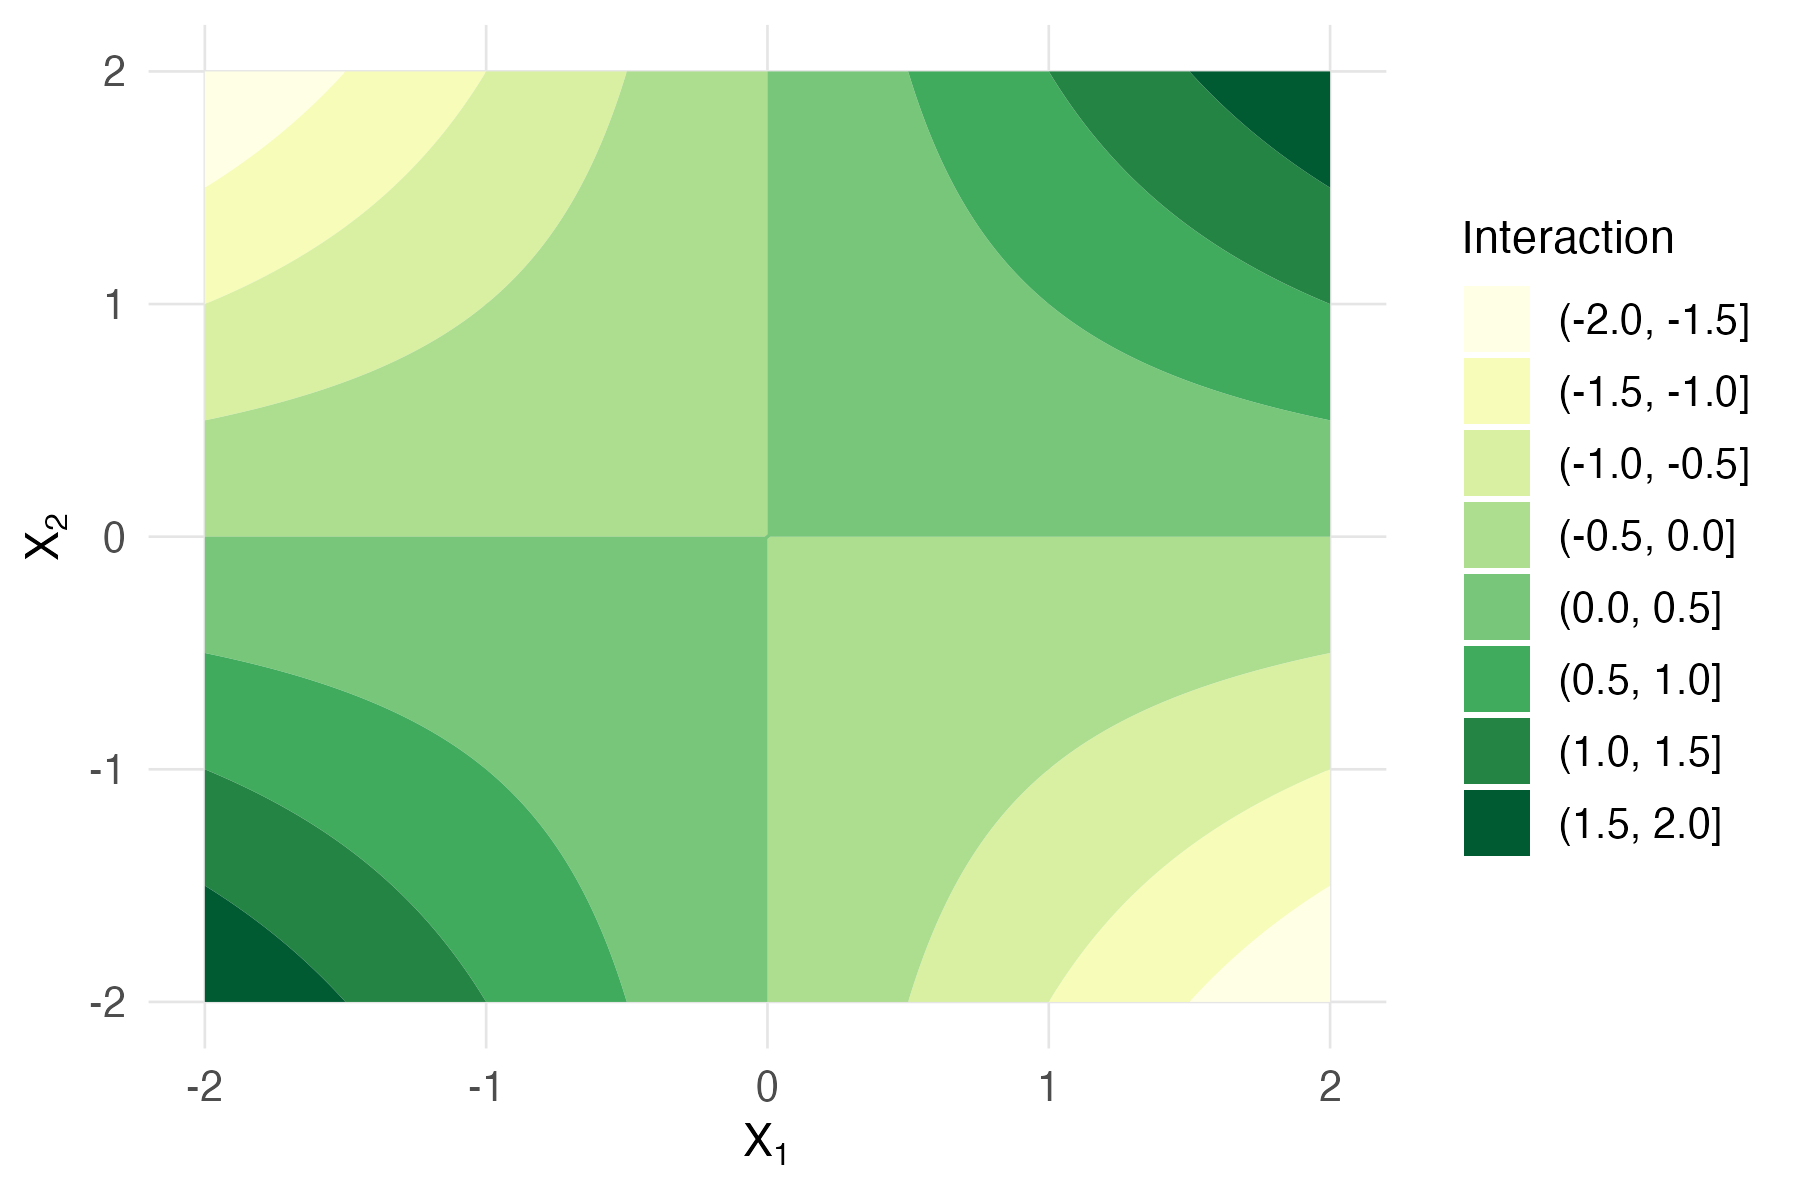
\includegraphics[width=\textwidth]{images/experiment_section/full_a1p20_a2p00_a11p10_a22p00_a12p05_rhop00_interaction.png}
        \end{minipage}
        \caption{Main and interaction effects for (1) $a_1 = 2$, $a_2 = 0$, 
                 $a_{11} = 1$, $a_{22} = 0$, $a_{12} = 0.5$, $\rho = 0$.}
    \end{subfigure}

    % -------- Pair 2 --------
    \begin{subfigure}[t]{\textwidth}
        \centering
        \begin{minipage}[t]{0.49\textwidth}
            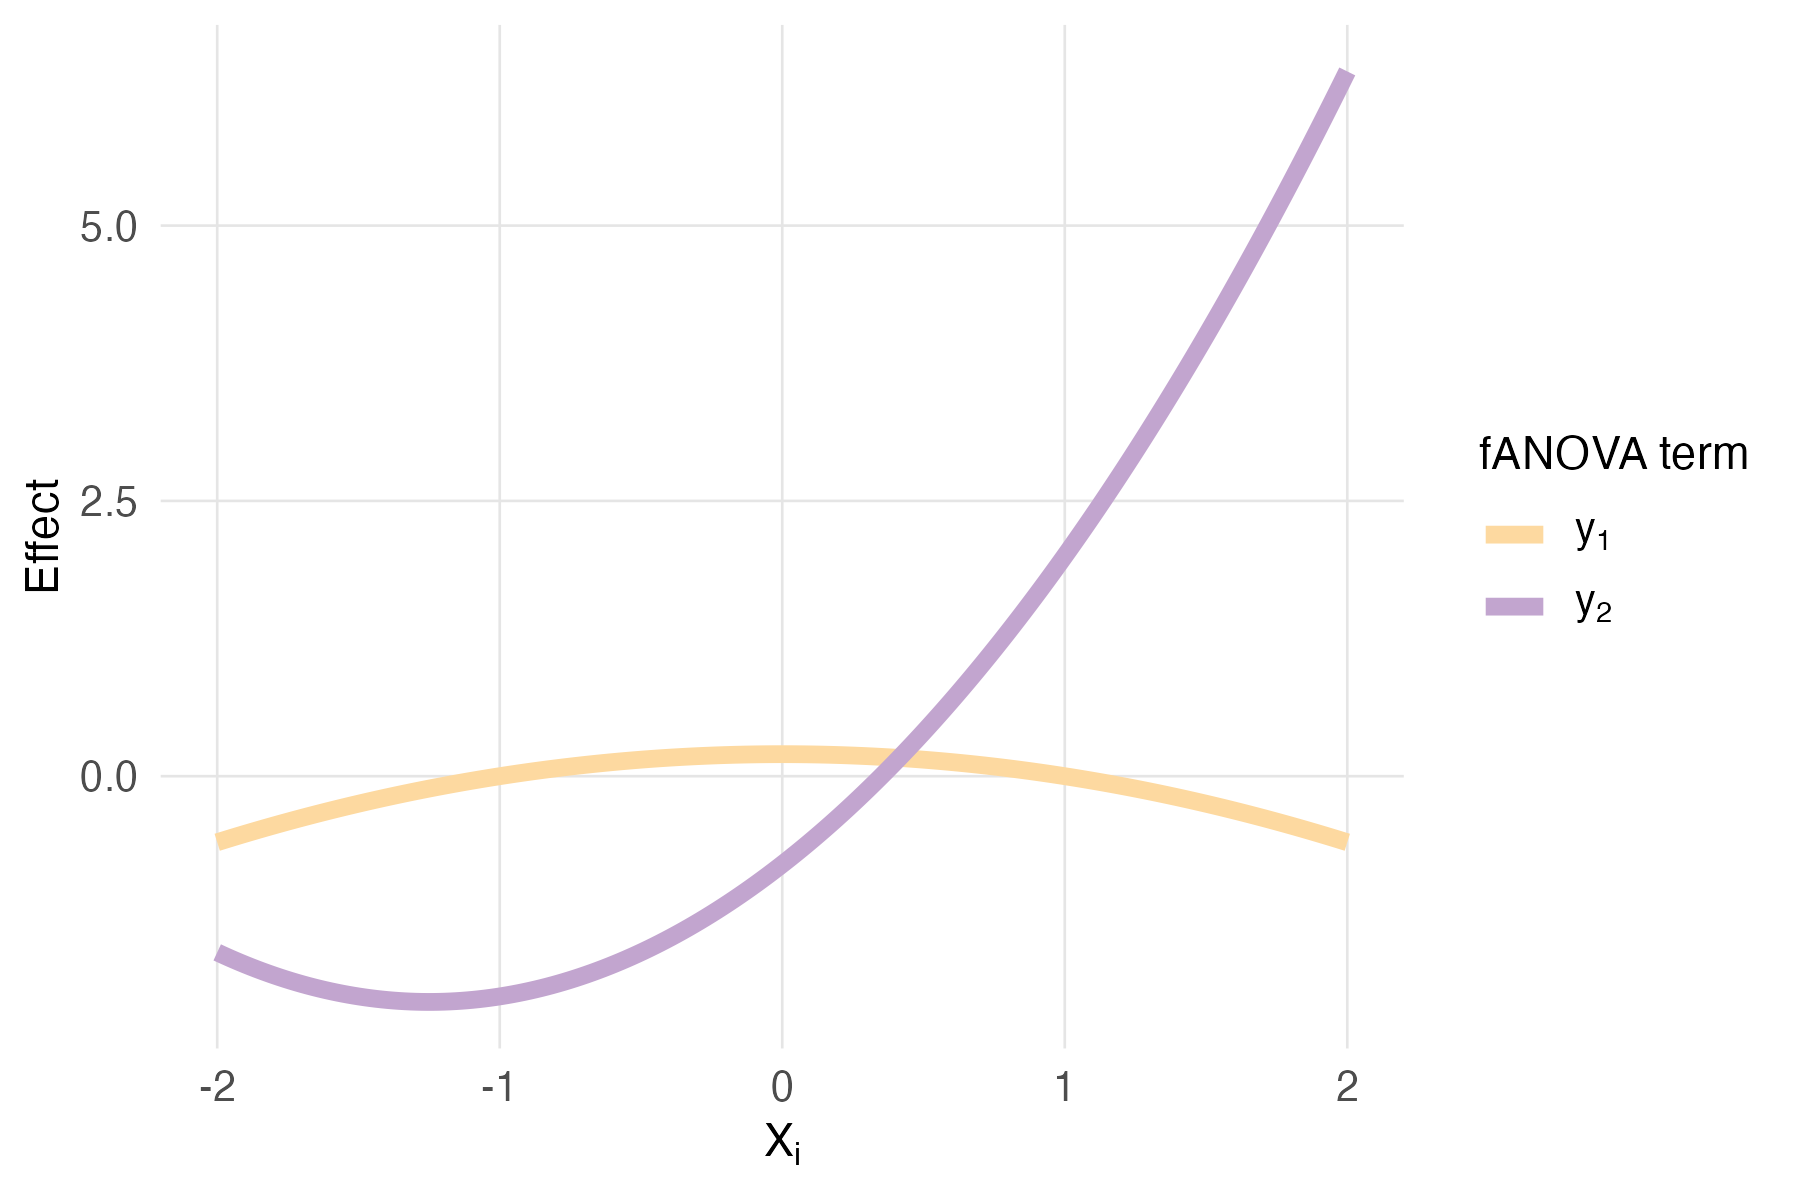
\includegraphics[width=\textwidth]{images/experiment_section/full_a1p00_a2p20_a11p00_a22p10_a12m05_rhop05_main.png}
        \end{minipage}%
        \hfill
        \begin{minipage}[t]{0.49\textwidth}
            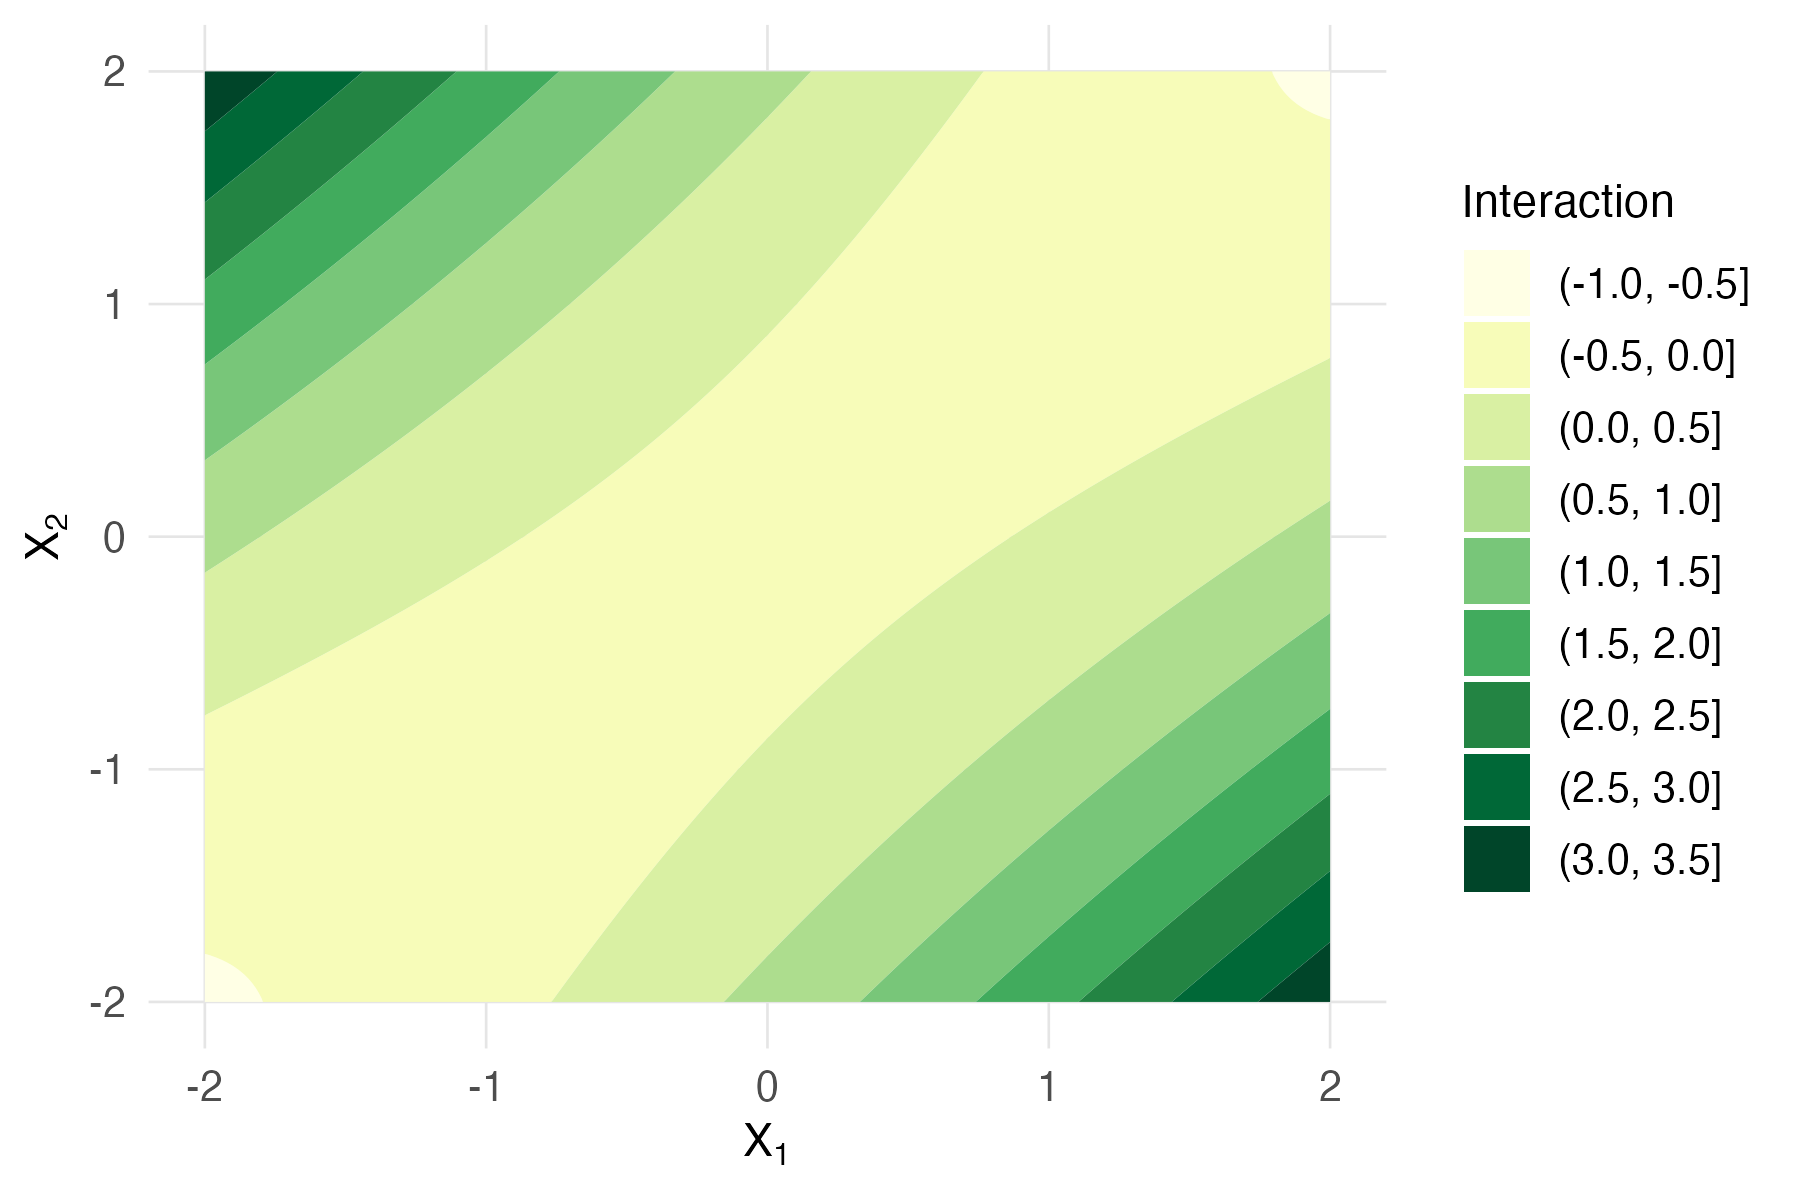
\includegraphics[width=\textwidth]{images/experiment_section/full_a1p00_a2p20_a11p00_a22p10_a12m05_rhop05_interaction.png}
        \end{minipage}
        \caption{Main and interaction effects for (2) $a_1 = 0$, $a_2 = 2$, 
                 $a_{11} = 0$, $a_{22} = 1$, $a_{12} = -0.5$, $\rho = 0.5$.}
    \end{subfigure}

    % -------- Pair 3 --------
    \begin{subfigure}[t]{\textwidth}
        \centering
        \begin{minipage}[t]{0.49\textwidth}
            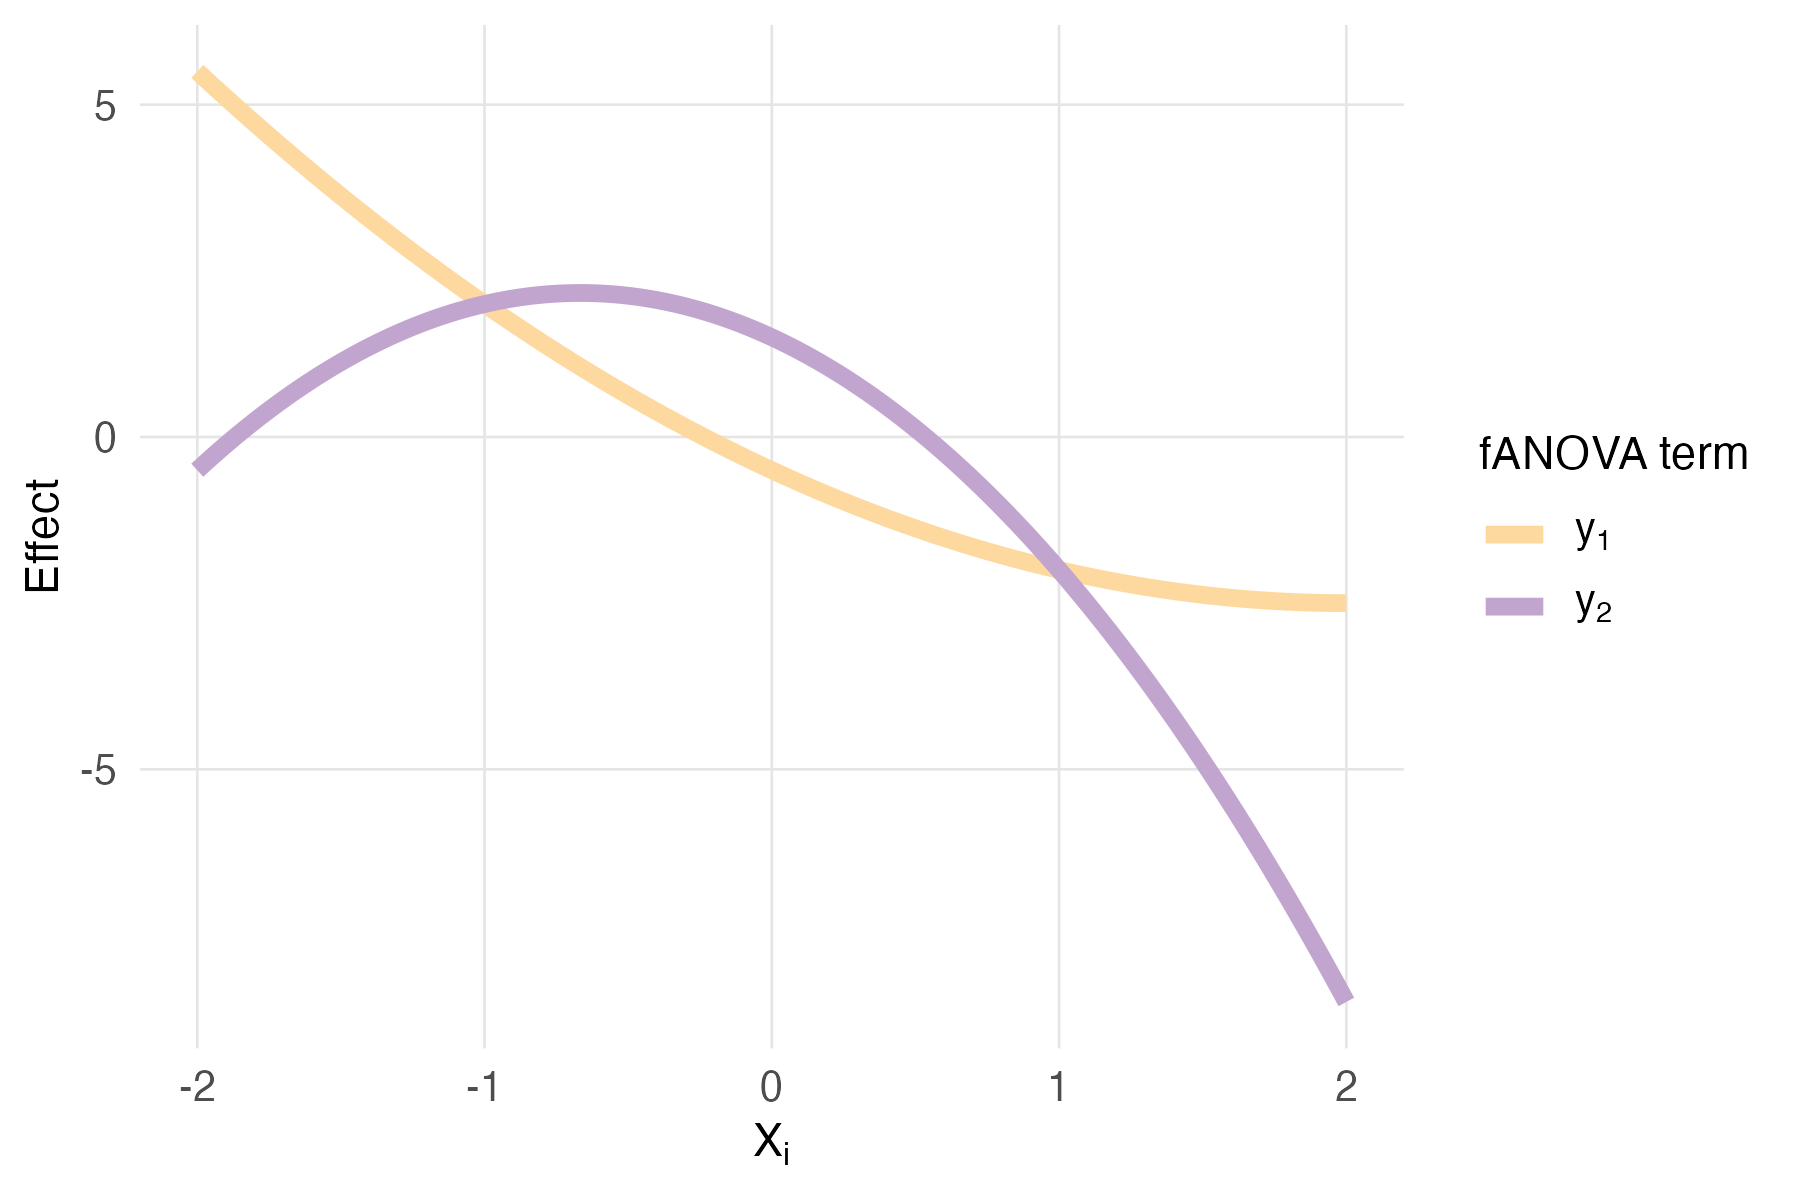
\includegraphics[width=\textwidth]{images/experiment_section/full_a1m20_a2m20_a11p10_a22m10_a12p10_rhom10_main.png}
        \end{minipage}%
        \hfill
        \begin{minipage}[t]{0.49\textwidth}
            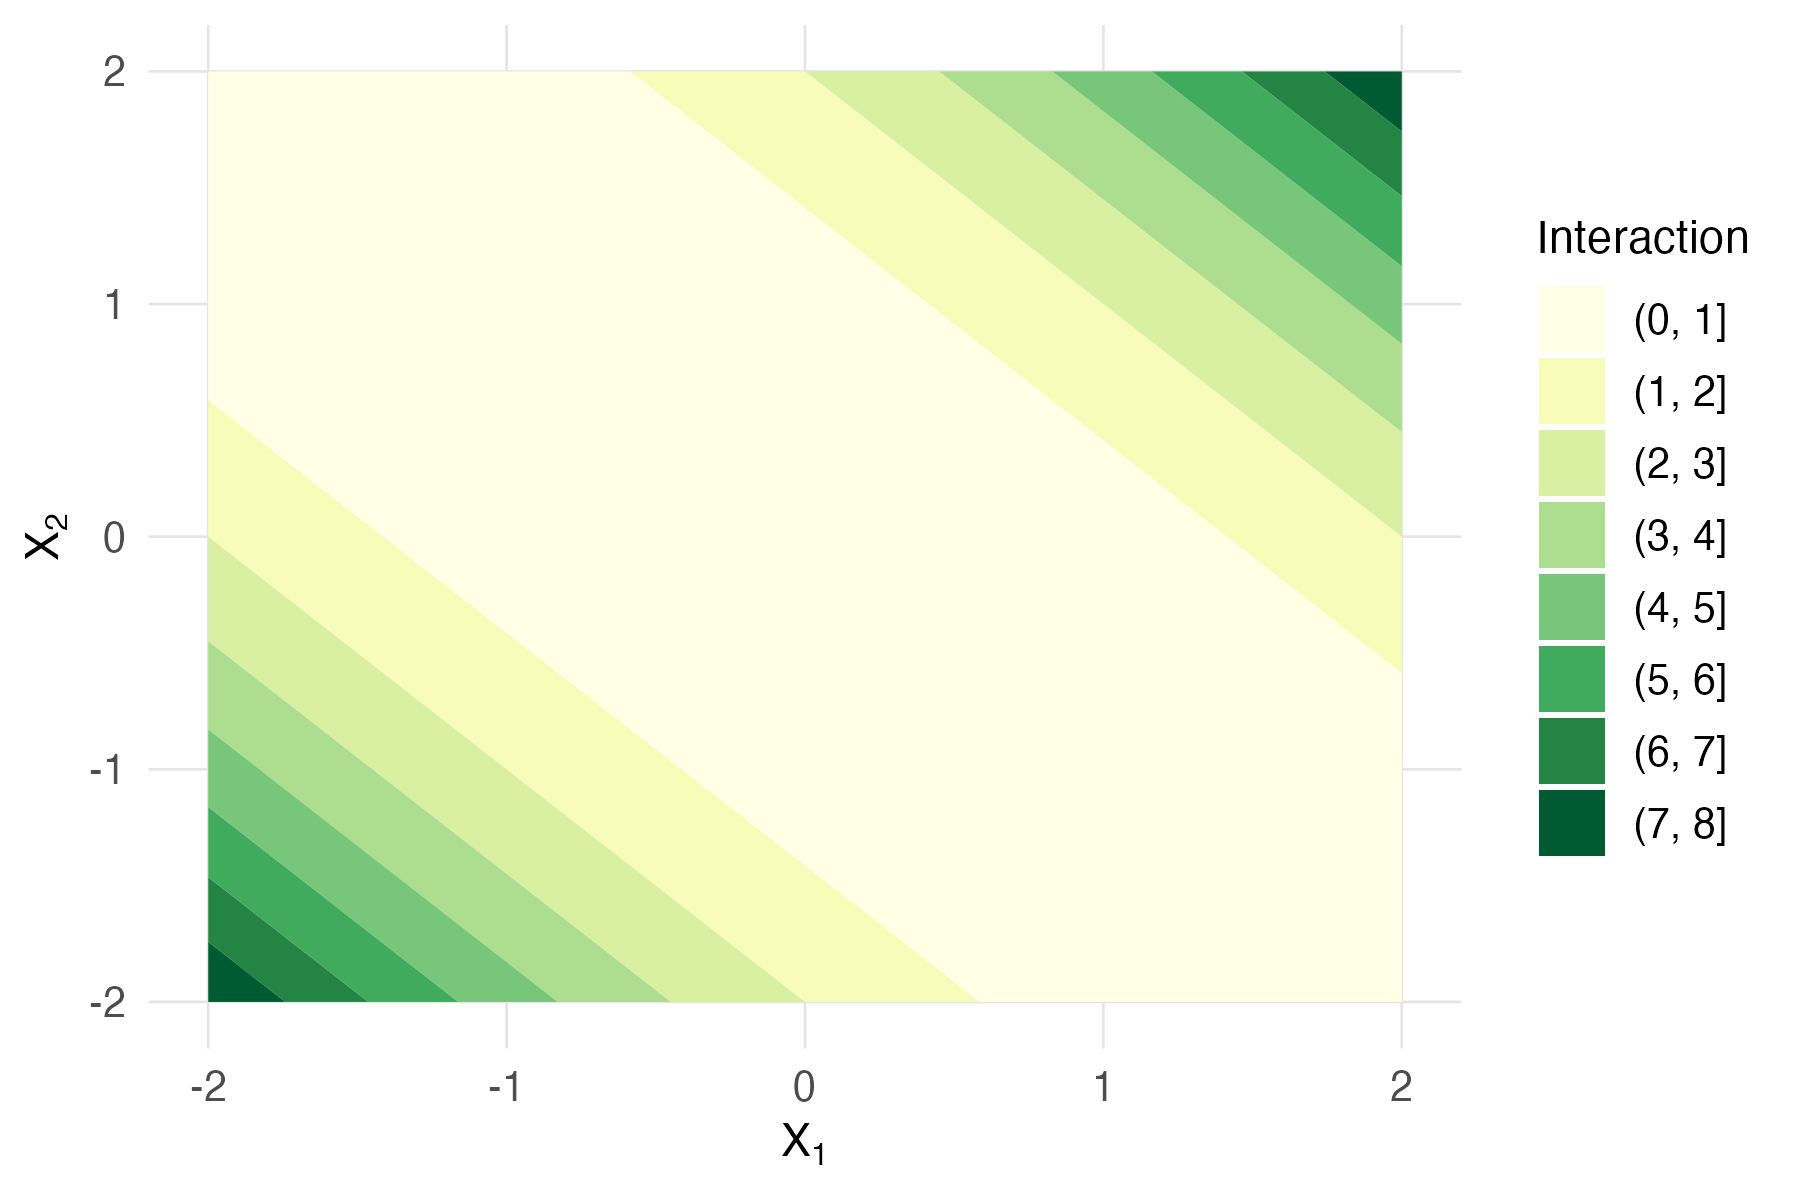
\includegraphics[width=\textwidth]{images/experiment_section/full_a1m20_a2m20_a11p10_a22m10_a12p10_rhom10_interaction.png}
        \end{minipage}
        \caption{Main and interaction effects for (3) $a_1 = -2$, $a_2 = -2$, 
                 $a_{11} = 1$, $a_{22} = -1$, $a_{12} = 1$, $\rho = -1$.}
    \end{subfigure}

    % -------- Pair 4 --------
    \begin{subfigure}[t]{\textwidth}
        \centering
        \begin{minipage}[t]{0.49\textwidth}
            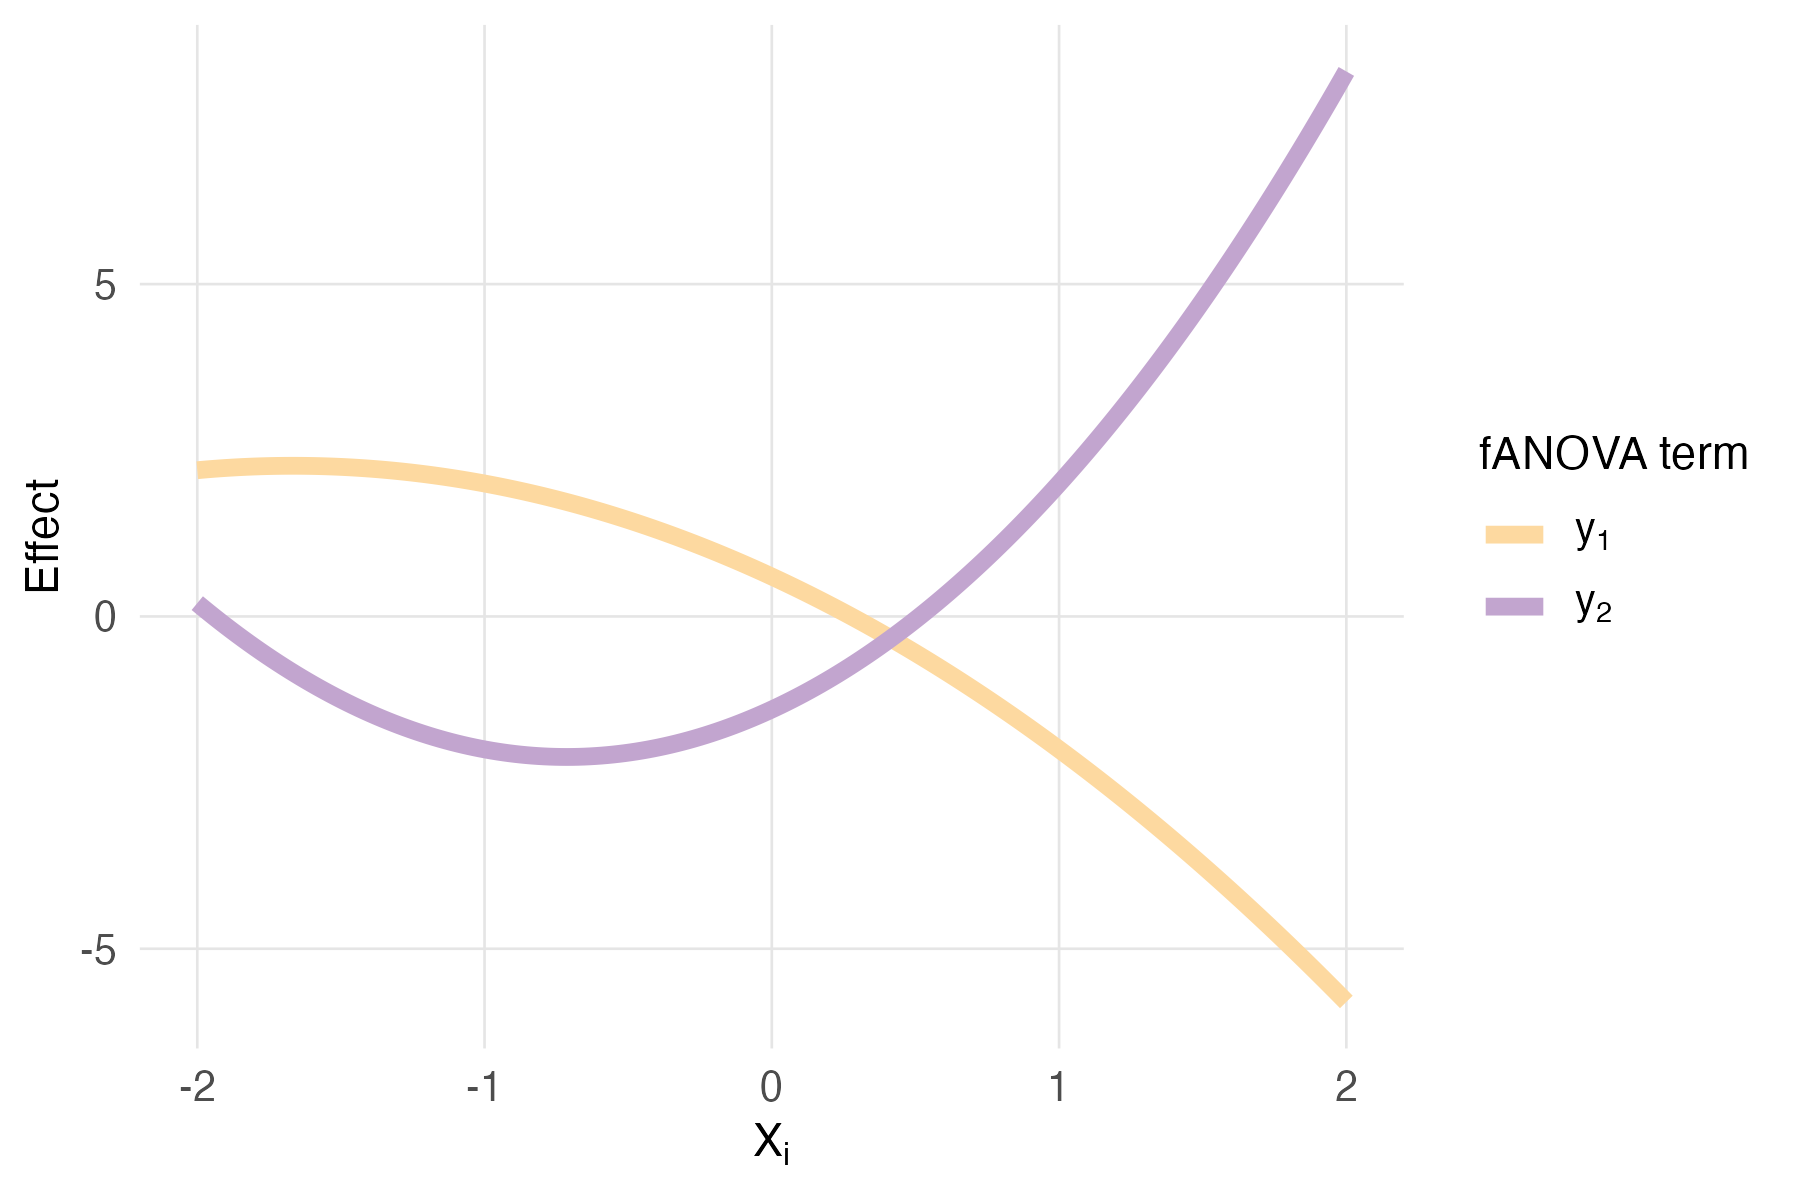
\includegraphics[width=\textwidth]{images/experiment_section/full_a1m20_a2p20_a11m10_a22p10_a12m10_rhom05_main.png}
        \end{minipage}%
        \hfill
        \begin{minipage}[t]{0.49\textwidth}
            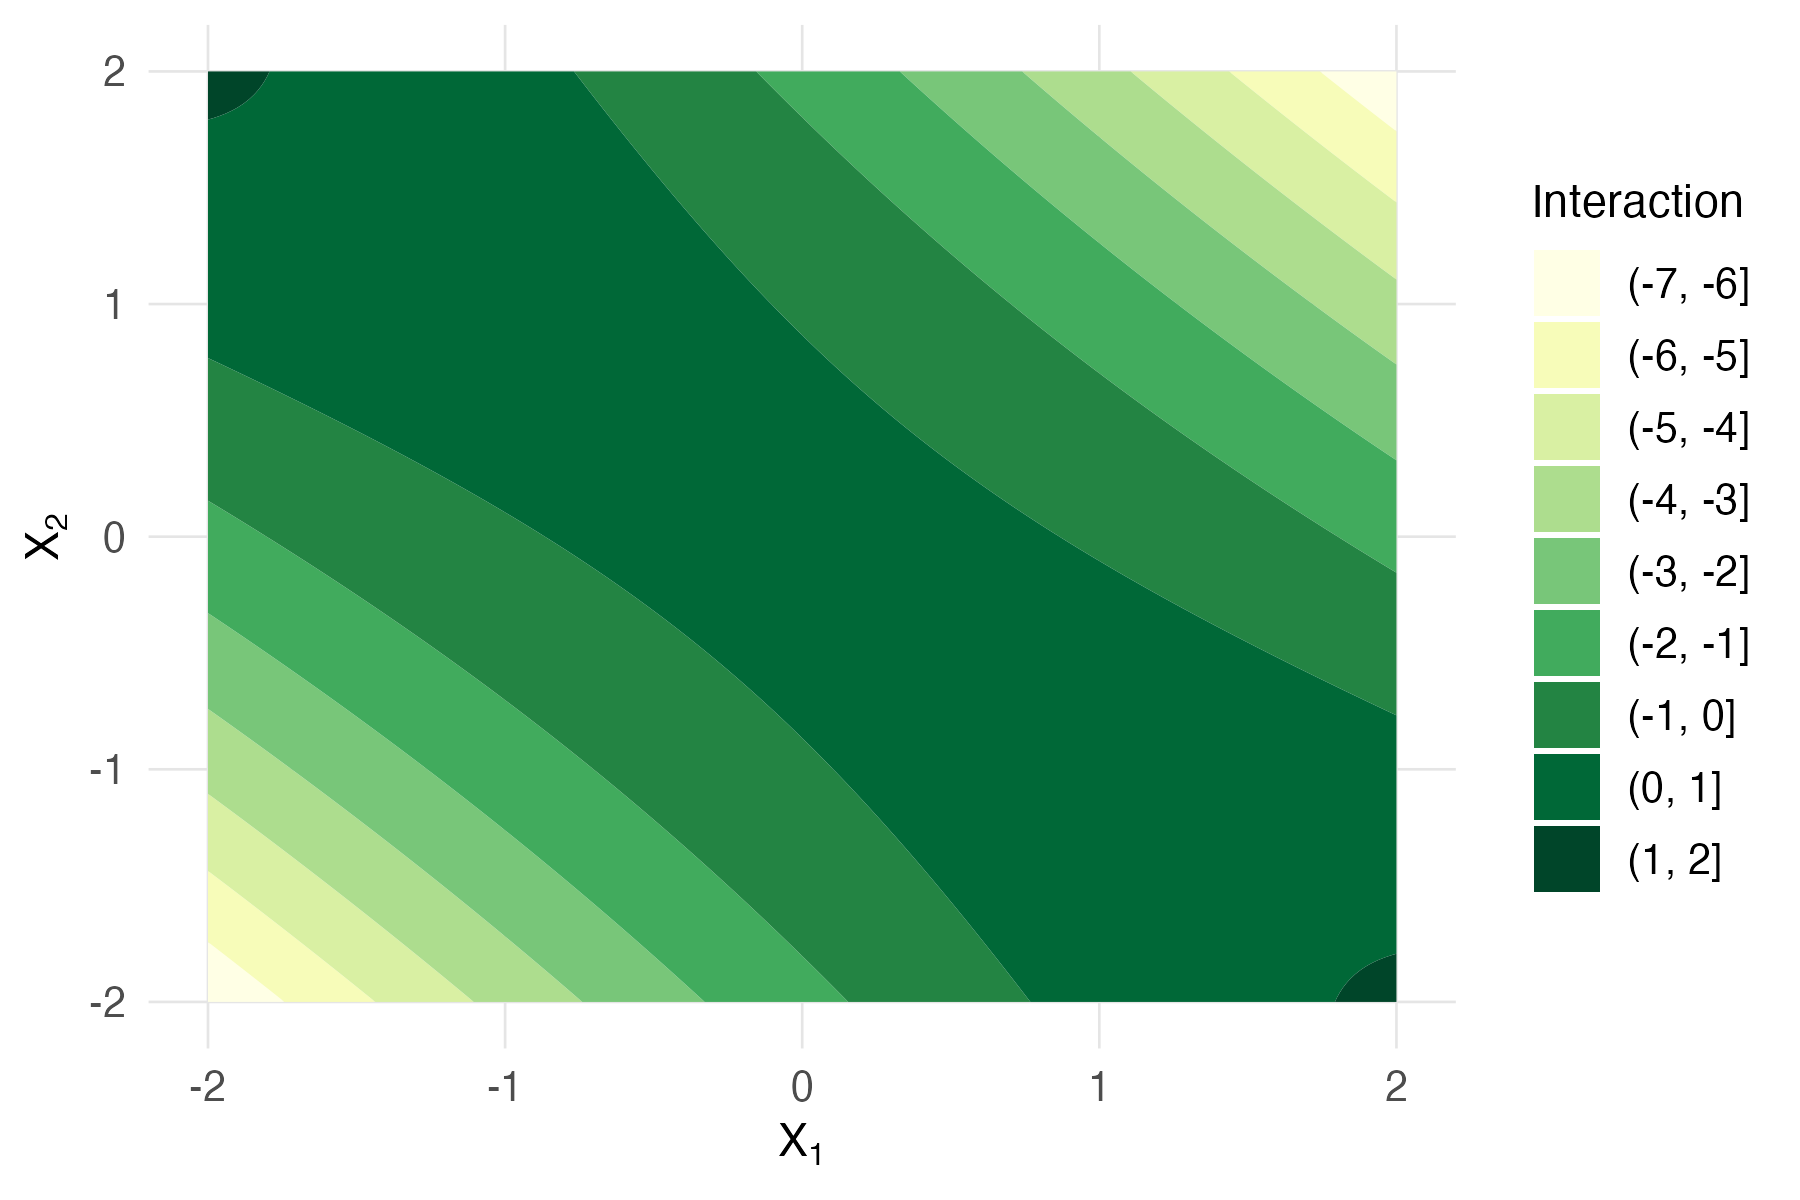
\includegraphics[width=\textwidth]{images/experiment_section/full_a1m20_a2p20_a11m10_a22p10_a12m10_rhom05_interaction.png}
        \end{minipage}
        \caption{Main and interaction effects for (4) $a_1 = -2$, $a_2 = 2$, 
                 $a_{11} = -1$, $a_{22} = 1$, $a_{12} = -1$, $\rho = -0.5$.}
    \end{subfigure}

    \caption{Main effects (left) and interaction contours (right) for four different \\ coefficient sets.}
    \label{fig:all_pairs_grouped}
\end{figure}

\subsubsection{Estimation of fANOVA components}
We want to end this thesis with a few words on estimation. This was all pretty theoretical and the examples we used foster understanding but they are toy examples and in reality the true function is unknown and more complex. So to become a more widely used, established interpretability method, an estimation scheme is inevitable.Current landscape of estimation approaches, We need more stable estimation approaches: Especially with real world blackbox models the individual components can be very complicated, probably no analytical closed form themselves
The fANOVA decomposition has a strong theoretical foundation but especially in modern work, estimation approaches and computational feasibility is an important aspect to consider.
Also, we saw that obtaining the fANOVA components analytically is not always possible, especially under dependent inputs. Therefore, we need to look at estimation approaches that allow us to compute the fANOVA components from data.\par

\textbf{Estimation based on Partial Dependence}. In his estimation framework \cite{hooker2004} picks up the role of projections in fANOVA. To obtain the component estimate for $y_u$, he proposes to estimate the projections of $y$ onto the subspace of variables spanned by $u$ empirically.
More concretely, one first estimates the conditional expected value of the variables in $u$ (keep variables in $u$ fixed an average over all others). This is a simple Monte Carlo estimation, which results in the partial dependence function (PD Function) for the variables in $u$ \citep{hooker2004}.
The PD Function can then be used to estimate the empirical projection of interest. He states that his method works well for functions that have a nearly additive true structure and purely additive functions are exactly recoverable with this approach. To save computational costs, he proposes to base the Monte Carlo estimates of the PD function on a randomly sampled subset of data points.
Problem: no true projections (under dependence or always?); extrapolation issues etc.; even if no product type measure assumption, still problems in handling dependent inputs.\par

\textbf{Estimation based on weighted least squares}. \cite{hooker2007} proposes a new estimation scheme for his generalized fANOVA decomposition. The mathematical problem one faces is more complex: the fANOVA components are defined in dependence of each other and system has to be solved simultaneously as we saw in the previous section.
Hooker rewrites the estimation problem as a restricted weighted least squares problem and solves it via Lagrange multiplier for the exact solution of the simultaneously defined generalized components; problem restricted to ensure hierarchical orthogonality.
The function is again evaluated at a grid of points to reduce the problem to a finite dimensional one. 
Because of the parallel to weighted least squares, it is also possible to compute a weighted standard ANOVA with existing software, but it is difficult to incorporate the constraints, so the components may not be hierarchical orthogonal.\par

None of these estimation approaches has a standard software implementation or published code. Some existing more or less finished implementations are numerically instable or yield illogical results. For our following experimental setup we therefore move within the range bivariate polynomials of degree two offer us and for which the solution is provided by Rahman.
